\documentclass[12pt]{article}
\usepackage{graphicx, subfigure, float, amsmath, amssymb, color}
\usepackage[margin = 1.0 in]{geometry}
\usepackage{natbib}

\renewcommand{\bottomfraction}{.9}
\renewcommand{\topfraction}{.9}
\renewcommand{\textfraction}{0.1}
\renewcommand{\floatpagefraction}{.9}



% definition of \customlabel, which is used to label supplementary figures and tables
\makeatletter
\newcommand{\customlabel}[2]{%
\protected@write \@auxout {}{\string \newlabel {#1}{{#2}{}}}}
\makeatother



\title{Amino-acid site variability among natural and designed proteins}
\author{Eleisha L.\ Jackson$^1$, Noah Ollikainen$^2$, Arthur W.\ Covert III$^1$,\\ Tanja Kortemme$^{2,3}$, and Claus O.\ Wilke$^1$}
\begin{document}

\date{\today}
\maketitle

\noindent
$^1$ Institute of Cellular and Molecular Biology, Center for Computational Biology and Bioinformatics, and Department of Integrative Biology, The University of Texas at Austin, Austin, Texas, USA\\
$^2$ Graduate Program in Bioinformatics,University of California San Francisco, San Francisco, California, USA\\
$^3$ California Institute for Quantitative Biosciences (QB3) and Department of Bioengineering and Therapeutic Science, University of California San Francisco, San Francisco, California, USA

\bigskip

\noindent
{\color{red}Text in red: Action items for Eleisha.}

\noindent
{\color{blue}Text in blue: Needs copy-editing.}

\noindent
{\color{green}Text in green: Misc. comments.}

%Use \textbf{} to bold tetxt
\begin{abstract}
Computational protein design attempts to create protein sequences that fold stably into pre-specified structures. Here we compare alignments of designed proteins to alignments of natural proteins, and assess how closely designed sequences recapitulate patterns of sequence variation found in natural protein sequences. We design proteins using Rosetta design, and we evaluate both fixed-backbone designs and variable-backbone designs with different amounts of backbone flexibility.

We find that proteins designed with a fixed backbone tend to underestimate the amount of site variability observed in natural proteins while proteins designed with an intermediate amount of backbone flexibility result in more realistic site variability. Proteins designed with an intermediate amount of backbone flexibility have amino acid distributions most similar to animo acid distributions observed in natural proteins. 
We find that in designed proteins the correlation between solvent exposure and site variability in designed proteins was lower than that in natural proteins suggesting that site variability is too uniform cross different solvent exposure sites (i.e. buried residues are too variability or exposed residues are too conserved). When comparing the amino acid frequencies in the designed proteins with the natural proteins we found that in the designed proteins hydrophobic residues were overrepresented. From these results we conclude that intermediate backbone flexibility during design results in more accurate protein design and that scoring functions that determine acceptable substitutions must improve to account for structural constraints on site variability patterns.
\end{abstract}

\section{Introduction}
\label{Introduction}

Computational protein design has made tremendous progress in recent years. For example, computational design has been used successfully to create proteins that bind to an influenza virus \citep{Fleishman2011}, to develop novel enzymes \citep{Rothlisberger2008}, and to develop novel protein folds not seen in nature example here \citep{Kuhlman2003}. All these examples have in common that many different computational designs were developed, and among the best were a few that worked experimentally. Thus, while computational design can produce specific sequences that fold correctly and are functional, it is much less clear how similar designed proteins are on average to natural proteins of comparable fold.

There are several patterns of sequence variation that are consistently seen in natural proteins. For example, amino acid frequencies follow characteristic distributions, and these distributions differ for surfaces and cores of proteins \citep{Overington1992,Porto2004,Bastolla2005,Moelbertetal2004}. In particular, hydrophobic residues tend to be more frequent in the core and polar residues tend to be more frequent on the surface. Further, sites in the core of a protein tend to be more conserved and to evolve slower than surface sites \citep{MirnyShakhnovich1999,Goldman1998,Bustamante2000,Conant2009,Franzosa2009,Ramsey2011,Scherreretal2012,MeyerWilke2012}. Presumably, sites in the core tend to be conserved because mutations at these sites are more likely to destablize the protein fold, due to steric clashes \citep{ChothiaFinkelstein1990}.

However, protein properties also vary systematically with factors related to the cellular environment in which proteins are expressed. For example, more highly expressed proteins tend to be more soluble and have less-sticky surfaces \citep{Tartagliaetal2007,Levyetal2012}. Current protein design algorithms optimize primarily for fold stability \citep{Butterfoss2006, Das2008}. Therefore, we would not expect them to reproduce any patterns caused by the cellular expression environment. By contrast, any patterns that are driven primarily by the requirement for sufficient fold stability, such as avoidance of steric clashes in the core, should be faithfully reproduced in computationally designed proteins.

Here, we carried out a systematic comparison between alignments of natural sequences and the corresponding alignments of designed sequences, for several different design conditions. We considered two distinct data sets, one of whole protein structures and one of individual protein domains. We analyzed which design conditions produced sequence alignments that were most similar to natural sequence alignments. We also analyzed by which parameters designed proteins differed the most from natural sequences. Overall, we found that proteins designed with a flexible backbone and using an intermediate amount of backbone flexibility were the most similar to natural proteins. However, substantial differences between designed and natural proteins remained even under the most advantageous design conditions. In particular, designed proteins tended to have too many polar and too few hydrophobic residues in the core, and they also tended to have cores that were too variable and/or surfaces that were too conserved. These trends were exacerbated for longer proteins.


\section{Methods}
\label{Methods}

\subsection{Data sets}

We analyzed two data sets, one of whole yeast proteins and one of protein domains. The yeast-proteins data set was taken from \citet{Ramsey2011} and comprised 38 protein structures homologous to an open reading frame in \emph{Saccharomyces cerevisiae}. For each of those structures, we had at least 50 homologous natural sequences, also taken from  \citet{Ramsey2011}. The protein-domain data set was taken from \citet{OllikainenKortemme} and comprised 40 protein domains. Only domains with at least one crystal structure in the Protein Database (PDB) and at least 500 sequences in the Pfam Database were selected for this data set. Domains were selected in order to represent several different types of protein folds and omains were also restricted to a length less than or equal to 150 amino acids. For each of these protein domains, we obtained alignments of homologous natural sequences from the Pfam database \citep{Pfam}, as described \citep{OllikainenKortemme}.

\subsection{Protein design}

For each structure in both data sets, we computationally designed 500 variants each, using multiple design methods. All design methods we used are implemented in the protein-design software Rosetta \citep{LeaverFayetal2011}. First, we used standard fixed-backbone design \citep{Kuhlman2003}. In this method, the protein backbone remains fixed and only amino-acid side chains are allowed to move. Second, we used the flexible-backbone method Backrub \citep{Smith2008}, which first generates an ensemble of alternative backbones and then designs side chains onto these backbones. The Backrub method takes as input a temperature parameter that determines the extent of backbone movements that occur during design. A temperature of zero corresponds to the fixed-backbone case while a temperature in excess of 1 allows substantial backbone movements. Here, we used temperatures spanning from 0.03 to 2.4. For the protein-domain data set, we also carried out one additional design method, called ``Soft''. This method which is similar to the fixed backbone method but the energy function used during sequence design dampens the weight of the repulsive Lennard-Jones (LJ) potential term \citep{OllikainenKortemme}.  Protein designs for the protein-domain data set have been previously published \citep{OllikainenKortemme}, while the designs for the yeast-proteins data set were newly generated for the present study.

\subsection{Data analysis}

We quantified the variability of sites in amino-acid alignments using site entropy $H_i$, defined as $H_i=\sum_{j}p_{ij}\ln p_{ij}$. Here, $p_{ij}$ is frequency of amino acid $j$ in alignment column $i$, and the sum runs over all amino acids. We compared amino-acid distributions of designed sequences to those of natural sequences using the Kullback-Leibler (KL) divergence. The KL divergence $D^\text{KL}_i$ is defined as $D^\text{KL}_i= \sum_j  p_{ij} \ln  (p_{ij}/q_{ij})$, where $q_{ij}$ is the frequency of amino acid $j$ in column $i$ of the reference alignment, and $p_{ij}$ is the corresponding frequency in the alignment that is being compared to the reference alignment. The sum runs over all amino acids.  When calculating frequencies used for the KL divergence we corrected for the presence of frequencies of zero by adding  $\frac{1}{20}$ to each amino acid count before calculating the frequencies. The KL divergence is inherently an asymmetric distance measure, comparing a probability distribution of interest to a reference distribution. Unless noted otherwise, we always used natural sequence alignments to calculate the reference frequencies $q_{ij}$ and designed sequence alignments to calculate the frequencies $p_{ij}$. Throughout this work, we calculated $D^\text{KL}_i$ separately at each site $i$ in a protein, and then averaged the $D^\text{KL}_i$ values for all sites in a protein to obtain a mean KL divergence for that protein. 

We calculated Relative Solvent Accessibility (RSA) of residues by first calculating the absolute Solvent Accessibility (SA) for each residue, using the software DSSP \citep{Kabsch1983}. For each protein, we extracted the chain of interest from the PDB structure and ran DSSP only on that chain. We calculated RSA by dividing the SA value for each residue by the maximum possible SA value, as given by \citet{Tien}. 

\section{Results}
\label{Results}


We wanted to assess the extent to which the sequence space of computationally designed proteins overlaps with the sequence space occupied by homologous natural proteins. Our general approach was to compare alignments of designed protein sequences to alignments of homologous natural sequences, for approximately 80 distinct protein structures. For each structure, we considered several different design methods (see Methods for details), and we designed 500 sequences for each structure and method. The protein structures we considered were subdivided into two distinct data sets, a data set of 38 yeast protein structures previously analyzed by \citet{Ramsey2011} and a data set of 40 protein domains previously analyzed by \citet{OllikainenKortemme}. Throughout this study, we analyzed these two data sets separately, because they corresponded to structures of substantially different sizes. The mean number of amino acids per structure was 215.4 in the yeast-proteins data set and 86.1 in the protein-domains data set.

\subsection{Overall site variability}
\label{SiteVariability}

We first compared overall amino-acid variability in designed and natural proteins. We assessed amino-acid variability at individual sites by calculating the entropy $H_i$ at each site $i$ in alignments of either designed or natural proteins. We then calculated the mean entropy over all sites in each alignment and used that quantity as a measure of the overall amino-acid variability in the alignment.

We found that protein design using a fixed backbone generally yielded insufficient site variability compared to natural sequences (Fig.~\ref{MeanEntropyComparison}).  This result was magnified in the smaller protein domains. In fact, for the protein domains, the most variable proteins under fixed-backbone design showed only about as much variability as the least variable natural proteins. Overall, there was a significant shift towards higher variability in natural proteins relative to proteins designed with fixed backbone (paired $t$ test, $P = 1.4\times10^{-10}$ for the yeast-proteins data set and $P<10^{-15}$ for the protein-domain data set). When switching from fixed-backbone design to variable-backbone design, we found that overall site variability increased. Further, site variability increased monotonously with the degree of backbone flexibility allowed during design, as measured by the design temperature (Fig.~\ref{MeanEntropyComparison}). At the highest temperatures, site variability in designed proteins consistently exceeded that of natural proteins. 

Proteins designed at intermediate temperatures had site variability that mostly closely resembled that of natural proteins. For the yeast-proteins data set, the temperature that provided the closest match was $T=0.03$, even though the variability of sequences designed at that temperature still exceeded the variability in natural sequences (paired $t$ test, $P= 0.0006$). For the protein-domains data set, the temperature that provided the closest match was $T=0.9$, for which variability was statistically indistinguishable from that found in natural sequence alignments (paired $t$ test, $P= 0.353$). However, for both data sets, natural sequences generally showed a larger spread in variabilities than did the designed sequences at the closest-matching temperatures (Brown-Forsythe test for equal variances, $P= 0.0003$ for the yeast-proteins data set at $T = 0.03$  and $P= 7.3\times 10^{-6}$ for the protein-domain data set at $T = 0.9$).

\subsection{Amino-acid distributions}
\label{AminoAcidDistributions}

We next compared amino-acid distributions between designed and natural sequences. First we looked at overall amino acid frequencies. We found that by-and-large, amino acid frequencies in designed proteins mirrored those in natural proteins (Figs.~\ref{AAFreqsYeastProteins} and \ref{AAFreqsProteinDomains}). The biggest differences arose in Cys, Pro, His, Trp, Phe, and Ala. Overall, we observed that hydrophobic residues tended to be under-represented in designed proteins whereas hydrophilic residues tended to be over-represented. This trend was stronger in the protein core than on the surface (Figs.~\ref{AAFreqsYeastProteins} and \ref{AAFreqsProteinDomains}). We also observed that the longer proteins in the yeast-proteins data set showed larger deviations between designed and natural sequences than the shorter proteins in the protein-domains data set. Finally, when comparing different design methods and design temperatures, we found that differences in amino-acid distributions were relatively minor (not shown).

Even if overall amino-acid distributions are approximately correct, the amino-acid distributions at individual sites can be poorly predicted \citep{Ramsey2011}. Therefore, we next compared, separately at each site, the similarity between amino-acid distributions in natural proteins and those in designed proteins. To carry out this comparison, we employed the Kullback-Leibler (KL) divergence \citep{Wasserman2004}, which measures how similar one probability distribution is to a reference distribution. A KL divergence of zero implies that the distributions are identical. The higher the KL divergence, the more dissimilar the focal distribution is to the reference distribution. (Note that KL divergence is not symmetric: if we swap the focal and the reference distribution, we will generally obtain a different KL divergence value.) We calculated the KL divergence at each site in each protein, and then averaged over sites within a protein to obtain a mean similarity score for each protein. As a control, we also randomly split the alignment of natural sequences for each protein structure into two halves and calculated the mean KL divergence of natural sequences against themselves.

First, in all comparisons, we found that the KL divergence of designed relative to natural sequences was much bigger than the KL divergence of natural sequences relative to themselves (Figs.~\ref{AADisFig1} and~\ref{NoahAADisFig1}). This finding indicates a substantial discrepancy between designed and natural sequences at individual sites. Second, we found that the mean KL divergence decreased with increasing design temperature (Figs.~\ref{AADisFig1}A and~\ref{NoahAADisFig1}A). Thus, according to the KL divergence measure, structures designed with the most flexible backbones had the most similar amino-acid distributions to those found in natural sequences.

However, the result that sequences designed at the highest temperatures are the most similar to natural sequences may be an artifact of the KL divergence measure. As design temperature increases, amino-acid variability increases, and amino-acid distributions become more uniform. A more uniform distribution is generally going to display more overlap with any given distribution than a more localized distribution, if the localized distribution is not correct. Thus, the decrease in KL divergence with increasing temperature may simply reflect the broadening of the distribution, not an actual improvement in reproducing natural amino-acid distributions. To assess whether amino-acid distributions in designed sequences were simply broadening with increasing temperature, or whether they were actually converging on the natural distributions, we carried out a second set of comparisons. We rank-ordered amino acids by frequency at each site in each protein, and then calculated the KL divergence of the rank-ordered distributions. This comparison considers only the shape of the distribution and does not assess whether the correct amino acids are present at individual sites. This second comparison generally found much lower KL divergence levels, even though still not as low as what was found for the control comparison of natural sequences with themselves (Figs.~\ref{AADisFig1}B and~\ref{NoahAADisFig1}B). 

More importantly, now KL divergence reached a minimum around a temperature of 0.3 (yeast proteins, Fig.~\ref{AADisFig1}B) to 1.2 (protein domains, Fig.~\ref{NoahAADisFig1}B) and rose again beyond that value. This finding indicates that higher design temperatures do not unequivocally produce more natural amino-acid distributions. Instead, there is an intermediate temperature, approximately coinciding with the temperature at which overall sequence variability matches best, at which amino acid distributions also are most similar.

\subsection{Site variability and solvent accessibility}
\label{ProteinStructure}

The previous analyses demonstrated that while designed proteins overall look similar to natural proteins, there are also important differences. We next wanted to identify whether these differences were present uniformly throughout the structure or could be located to specific structural regions. In our analysis of amino-acid distributions, we had already seen that amino-acid distributions seemed to deviate more at buried sites than at exposed sites (Figs.~\ref{AAFreqsYeastProteins} and~\ref{AAFreqsProteinDomains}).

We first plotted site variability against relative solvent accessibility (RSA, a dimensionless number from 0 to 1 measuring the relative solvent exposure of individual residues) for individual proteins. See Fig.~\ref{Entropy_vs_RSA_example} for one example. We generally found that site variability displayed a substantial spread even for sites of very similar RSA. At the same time, there was an overall trend for sites with higher RSA to be more variable than sites with lower RSA. This trend was generally stronger in flexible backbone designs than in fixed backbone designs (Fig.~\ref{Entropy_vs_RSA_example}). To analyze the relationship between site variability and RSA more systematically, we calculated the correlation between these two quantities for all proteins (Figs.~\ref{Correlation_figure} and~\ref{Correlation_figure_Noah}). On average, natural sequence alignments showed a higher correlation than alignments of designed sequences, regardless of design method. 

Intermediate design temperatures showed the highest correlations, but correlations were nevertheless significantly lower in designed proteins than in natural proteins (paired $t$ test, $P=3.78\times 10^{-10}$ [$T=0.3$, yeast proteins] and $P= 2.10\times 10^{-5}$ [$T=0.3$, protein domains]).  We also investigated whether the designed proteins with the highest correlations corresponded to the natural proteins with the highest correlations, and found this generally to be the case (Figs.~\ref{Correlation_figure}B and~\ref{Correlation_figure_Noah}B).

Our finding that correlations between site entropy and RSA are lower in designed proteins than in natural proteins indicates that, in designed proteins, site variability is too uniform across different solvent exposure states. In short, designed proteins are either too variable in the core or too conserved on the surface. To obtain a clearer picture of how exactly designed proteins differed from natural proteins, we once more considered the distributions of mean site entropies, but now calculated separately for buried sites ($\text{RSA}\leq0.05$), for partially buried sites ($0.05<\text{RSA}\leq0.25$), and for exposed sites ($\text{RSA}>0.25$). Figure~\ref{Mean_Entropy_Surface_Core} shows the medians of these distributions. For designed proteins, the mean site variabilities of exposed and of partially buried sites are close in magnitude while the mean site variabilities of buried sites are generally consistently lower. By contrast, in natural sequences exposed sites show much more variability than partially buried sites.

If buried sites are too variable or exposed sites too conserved in designed proteins, we reasoned that hybrid designs, in which buried sites were taken from sequences designed at a lower temperature and exposed sites from sequences designed at a higher temperature, should display correlations more similar to those seen in natural proteins. 

According to Fig.~\ref{Mean_Entropy_Surface_Core}, for the yeast proteins buried and partially buried sites in designed proteins had site variability most similar to that of natural sequences in proteins designed with a fixed backbone or in proteins design temperature of $T=0.03$. In the protein-domains data set, that temperature was $T=0.3$ to $T = 0.6$.  By contrast, for exposed sites the site variability in designed proteins was most similar to that of natural sequences at a design temperature of $T= 0.1$ (yeast proteins) and $T  = 1.2$ (protein domains).  We thus built our hybrid designs by combining sites from these temperatures. We found that the distribution of the site-entropy--RSA correlations in hybrid designs was comparable to that in natural sequences (Fig.~\ref{Mixed_RSA_Entropy}). However, predictions for specific proteins lacked accuracy (Fig.~\ref{Mixed_Entropy_Correlation_Plot}).


\section{Discussion}

We have compared site variability and amino-acid distributions in designed and natural proteins, for two distinct data sets. One data set consisted of 38 yeast proteins, and the other consisted of 40 protein domains. Structures in the yeast-proteins data set were, on average, much larger than structures in the protein-domain data set, while alignments of natural sequences in the protein-domain data set were somewhat more variable than those in the yeast-proteins data set. We have found that proteins designed with a flexible backbone, using an intermediate design temperature, were generally the most similar to natural proteins. Overall amino-acid frequencies in designed proteins were similar, though not identical, to those in natural proteins. However, amino-acid frequencies at individual sites showed substantial deviations. Finally, we have found that site variabilities in designed proteins are too uniform across different solvent exposure states of residues. Designed proteins have either cores that are too variable or surfaces that are too conserved.

In previous studies, native sequence recovery has been used to assess design accuracy \citep{Ganinza2012, Barth2007}. Native sequence recovery is defined as the mean percent of native amino acid identities that are that are observed in the designed sequence. Despite its widespread use, native sequence recovery may not always been a good indicator of design accuracy, especially when examining different sequences that are compatible with one specific structure. A major goal of design is to find sequences that fold into a specific structure. For this goal, one designs a series of structural ensembles that are similar to the native structure and then identifies low energy sequences for each of these designed ensembles. Sequence recovery is not necessarily a good indicator of design accuracy in this case, because these sequences while folding the desired structure, may not necessarily have a high sequence similarity with the sequence of the native structure.  For this reason, we believe that it is important to assess design accuracy by multiple different methods, as we have done here.

A previous study, the source of the protein-domains data set we analyzed here, has similarly considered multiple measures of design accuracy \citep{OllikainenKortemme}. Specifically, that work considered sequence sequence entropy, profile similarity, and amino acid co-variation between designed and natural proteins. Sequence entropy for each site was calculated as done here. They used profile similarity to account for similarities in amino acid distributions as opposed to our measurement of using KL Divergence to quantity amino acid distributions. The profile similarity score was calculated as the mean prof\_sim score between two corresponding sites within the designed and natural proteins as calculated in \citet{Yona2002}. The prof\_sim score is calculated from two factors: the \textit{a priori} probability that the distributions resemble the same source distribution and the statistical similarity of amino acid the distributions of the two protein alignments. The same set of protein domains was used in our analysis. Although the optimal design temperature changed according to the comparison method, both analyses found that intermediate backbone flexibility resulted in protein designs that were the most similar to natural proteins.

We analyzed two distinct datasets. One contained 40 protein domains. These protein domains were constrained to be less than 150 amino acids in length and had a mean length of 86.1 amino acids. The other was comprised of 38 whole yeast proteins, with a mean length of 215.4 amino acids. For each structure in each data set, we had an associated alignment of natural sequences to assess natural variability for that structure. (Note that sequences homologous to the yeast proteins were not constrained to be fungal sequences.) Sequence alignments in the protein-domain data set were somewhat more variable than sequence domains in the yeast-protein data set. We found that optimal design temperatures were lower for the yeast-protein data set than for the protein-domains data set. This finding is consistent with both increased mean length and reduced mean variability in the yeast-protein data set relative to the protein-domains data set. In particular, large cores in the larger proteins may lead to larger conserved regions whose site variability patterns are better recaptured at lower design temperatures. 

We found generally that designed protein sequences are similar but by no means identical to natural sequences. To some extent, this discrepancy is to be expected. Designed protein sequences are optimized entirely for thermodynamic stability. Natural proteins experience a variety of selective pressures, stability being only one of them. For example, natural proteins experience selection pressures for native protein--protein interactions, against non-specific protein--protein interactions, and against misfolding and aggregation  \citep{Fraser2002, Zarrinpar2003, Drummond2008}{\color{red}more refs}. If they are enzymes, natural proteins also require the appropriate mutations that guarantee enzymatic activity, even if those mutations are thermodynamically destabilizing \citep{Bloometal2006}. While selection for enzymatic activity will likely affect only a few sites in a protein, the other selective forces (misfolding, aggregation, native and non-specific interactions) have the potential to exert much broader selection pressures across many sites in a protein. As long as design algorithms do not take these selection pressures into account, we cannot expect design algorithms to reproduce natural sequence variation exactly.

To identify at what sites discrepancies between natural and designed proteins arose, we explicitly examined the relationship between structure and sequence variability. In particular, we analyzed the correlation between RSA and site entropy, which reflects the well-known observation that proteins are more variable on the surface than in the core. We found that the difference between surface and core variability was much more pronounced in natural proteins than in designed proteins. Designed proteins either have surfaces that are too variable or cores that are too conserved. We created hybrid designs, taking core sites from one set of designed proteins and surface site from another set, designed with more backbone movement, and tested whether these hybrid designs showed the appropriate differential in variability between core and surface sites. We found that they did so as a population (Fig.~\ref{Mixed_RSA_Entropy} but not individually (Fig.~\ref{Mixed_Entropy_Correlation_Plot}). This observation indicates that there is some aspect of protein fold stability that differentially affects surface and core residues and that is not yet properly incorporated into current design algorithms. Simply raising the design temperature on the surface but not in the core is not sufficient to capture this effect.

{\color{green}Tanja, we're just making stuff up here:} For both data sets, the designed proteins had fewer hydrophobic residues and more polar residues than expected from natural sequence alignments. This trend was particularly apparent in the protein core, and it was more extreme for larger proteins. These discrepancies suggest a need for further improvement of the design algorithm, most likely the scoring function. Rosetta uses a scoring function that predicts the energy of a given sequence folded into a particular target structure \citep{Das2008}. As a component of this scoring function, Rosetta uses reference energies for each amino acid to control for amino acid composition within the designed sequences \citep{Jacak2012}. These energies favor more polar protein surfaces and control for surface hydrophobicity. Improvements to these parameters or modifications to the way the scoring function handles hydrophobicity on the surface or the core might further improve the design algorithm. In particular, it might be necessary to use different parameterizations for small and for large proteins. There could also be improvements in the design algorithm that better address core packing. Methods such as RosettaHoles \citep{Sheffler2009} that allow for assessment of protein core packing can been used in future algorithm refinement.

In our analysis of approximately 80 protein structures, we found that proteins designed with an intermediate amount of backbone flexibility exhibited site-variability patterns most closely resembling that of natural proteins.  However, the optimal range of backbone flexibility depended on protein size. Further, even when the overall site variability matched that of natural sequences, the specific amino-acid distributions at individual sites did not match that well, as quantified by the relatively large KL divergence values between natural and designed alignments. Similarly, intermediate design temperatures showed the highest correlation between RSA and site variability (as measured by entropy). However, even at the optimal design temperature ($T \sim 0.3$ for both data sets), the designed proteins exhibited systematically lower correlations than did the natural proteins. Consequently, using current state-of-the-art design algorithms, designed proteins have either surfaces that are too conserved or cores that too variable. We suspect that just adjusting reference energies, as discussed in the previous paragraph with regards to amino-acid frequencies, would likely not be sufficient to address this issue. Instead, we see a need for improved flexible-backbone design algorithms that can generate larger backbone movements on the surface without disturbing the core backbone as much.



\section{Acknowledgments}

This work was supported in part by NIH grant R01 GM088344 and by {\color{red}DTRA ...}

\bibliographystyle{peerj} %"style
\bibliography{ProjectBib} %expected file "my refs.bib"

\cleardoublepage

\section{Figures}

\begin{figure}[H]
%\centerline{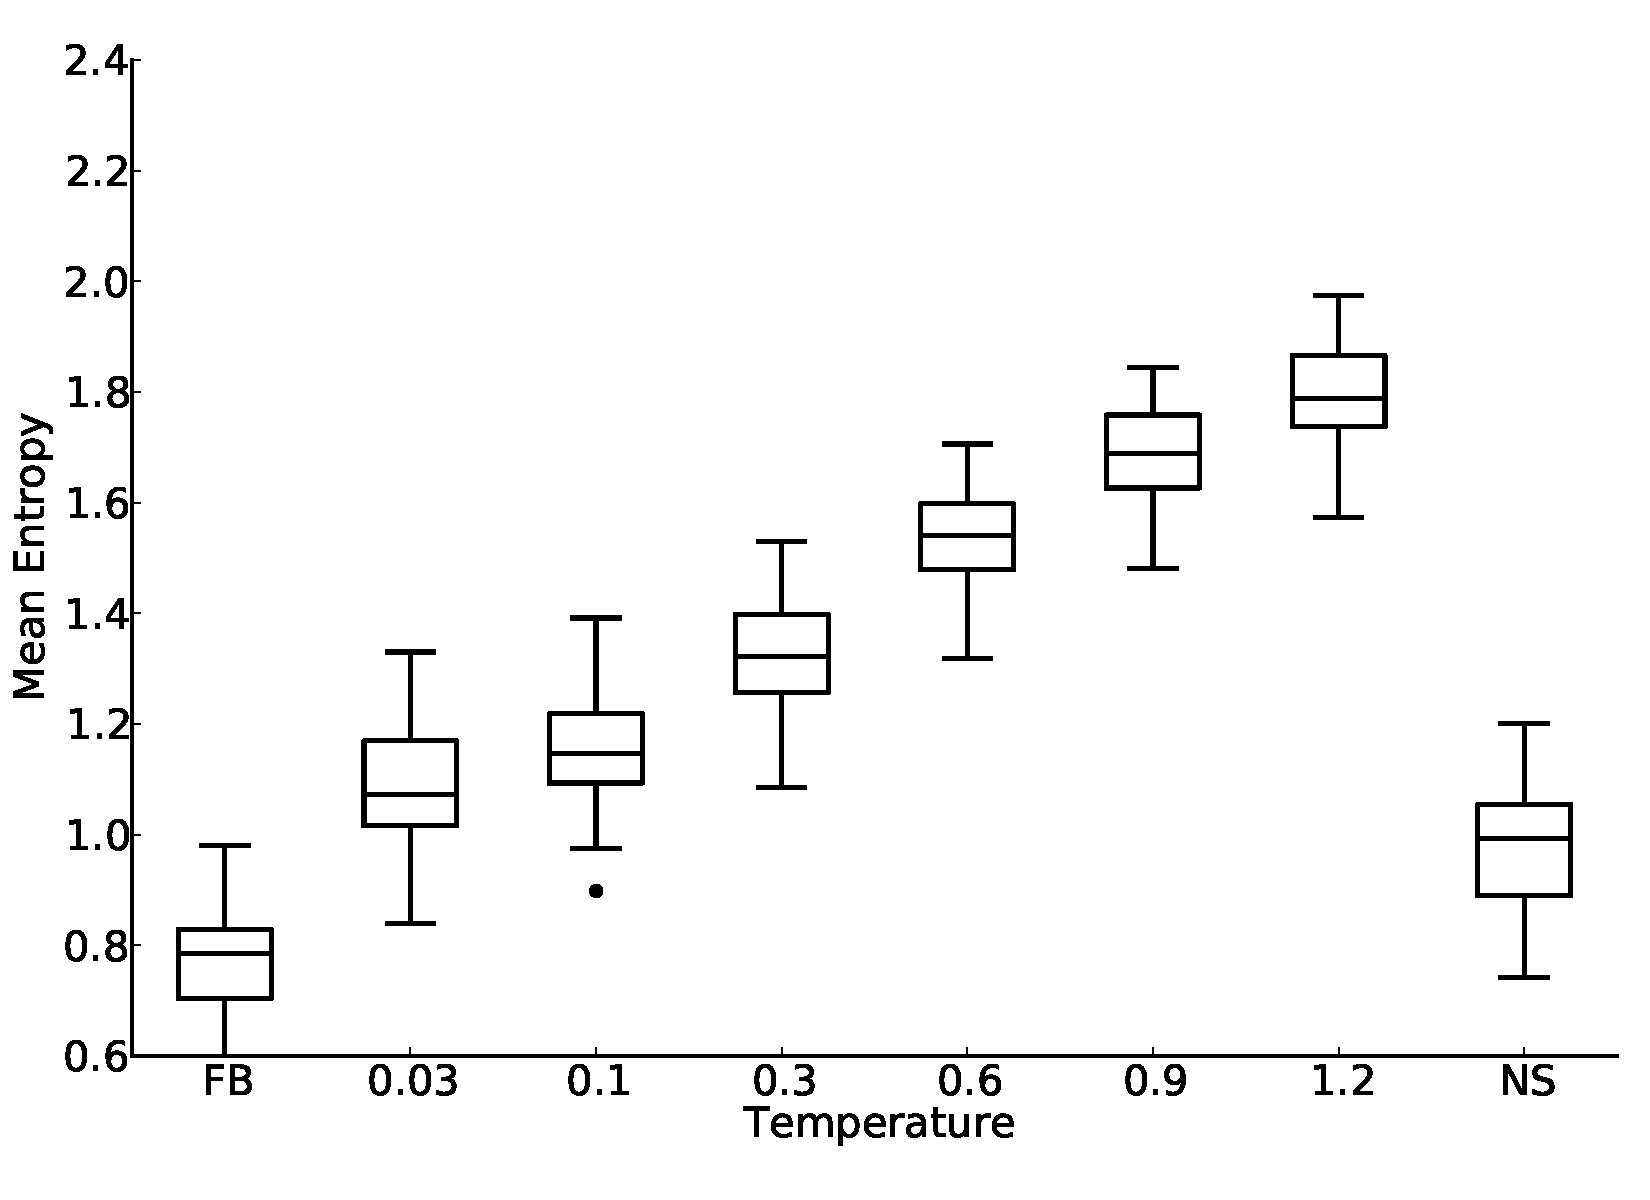
\includegraphics[width = 3in]{figures/Mean_Entropy_vs_Temp_Boxplot.pdf}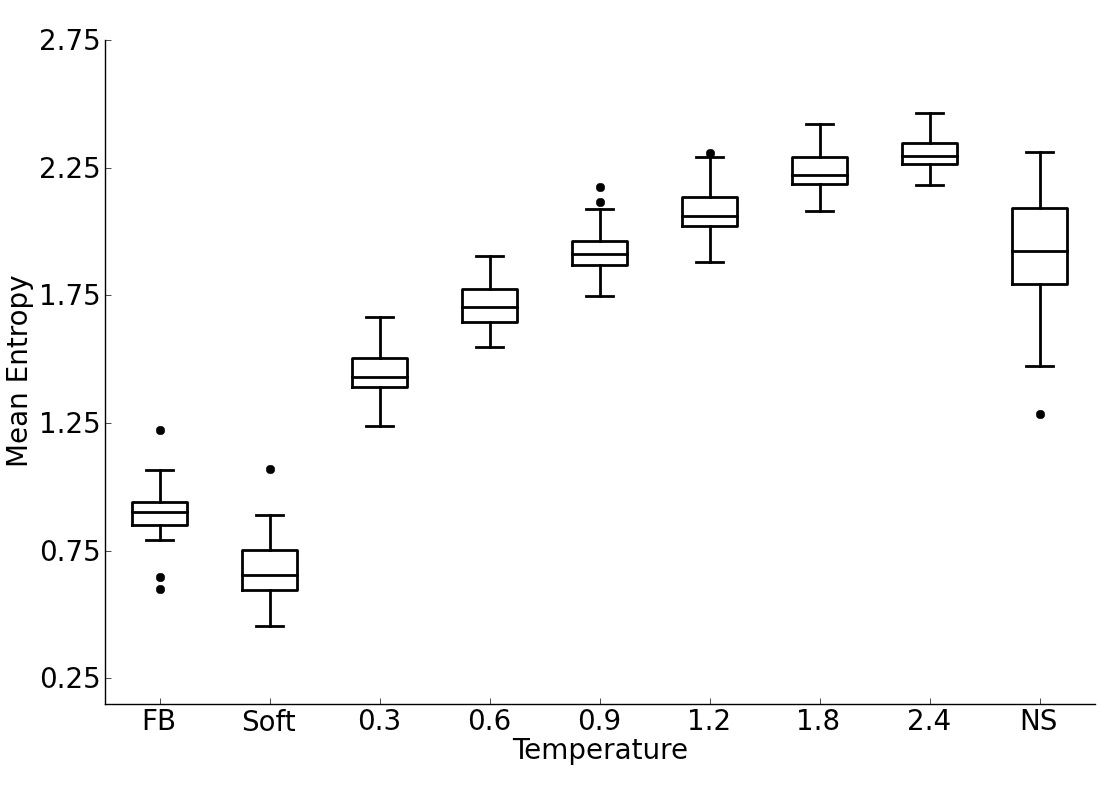
\includegraphics[width = 3in]{figures/Mean_Entropy_vs_Temp_Boxplot_Noah.pdf}}
\centerline{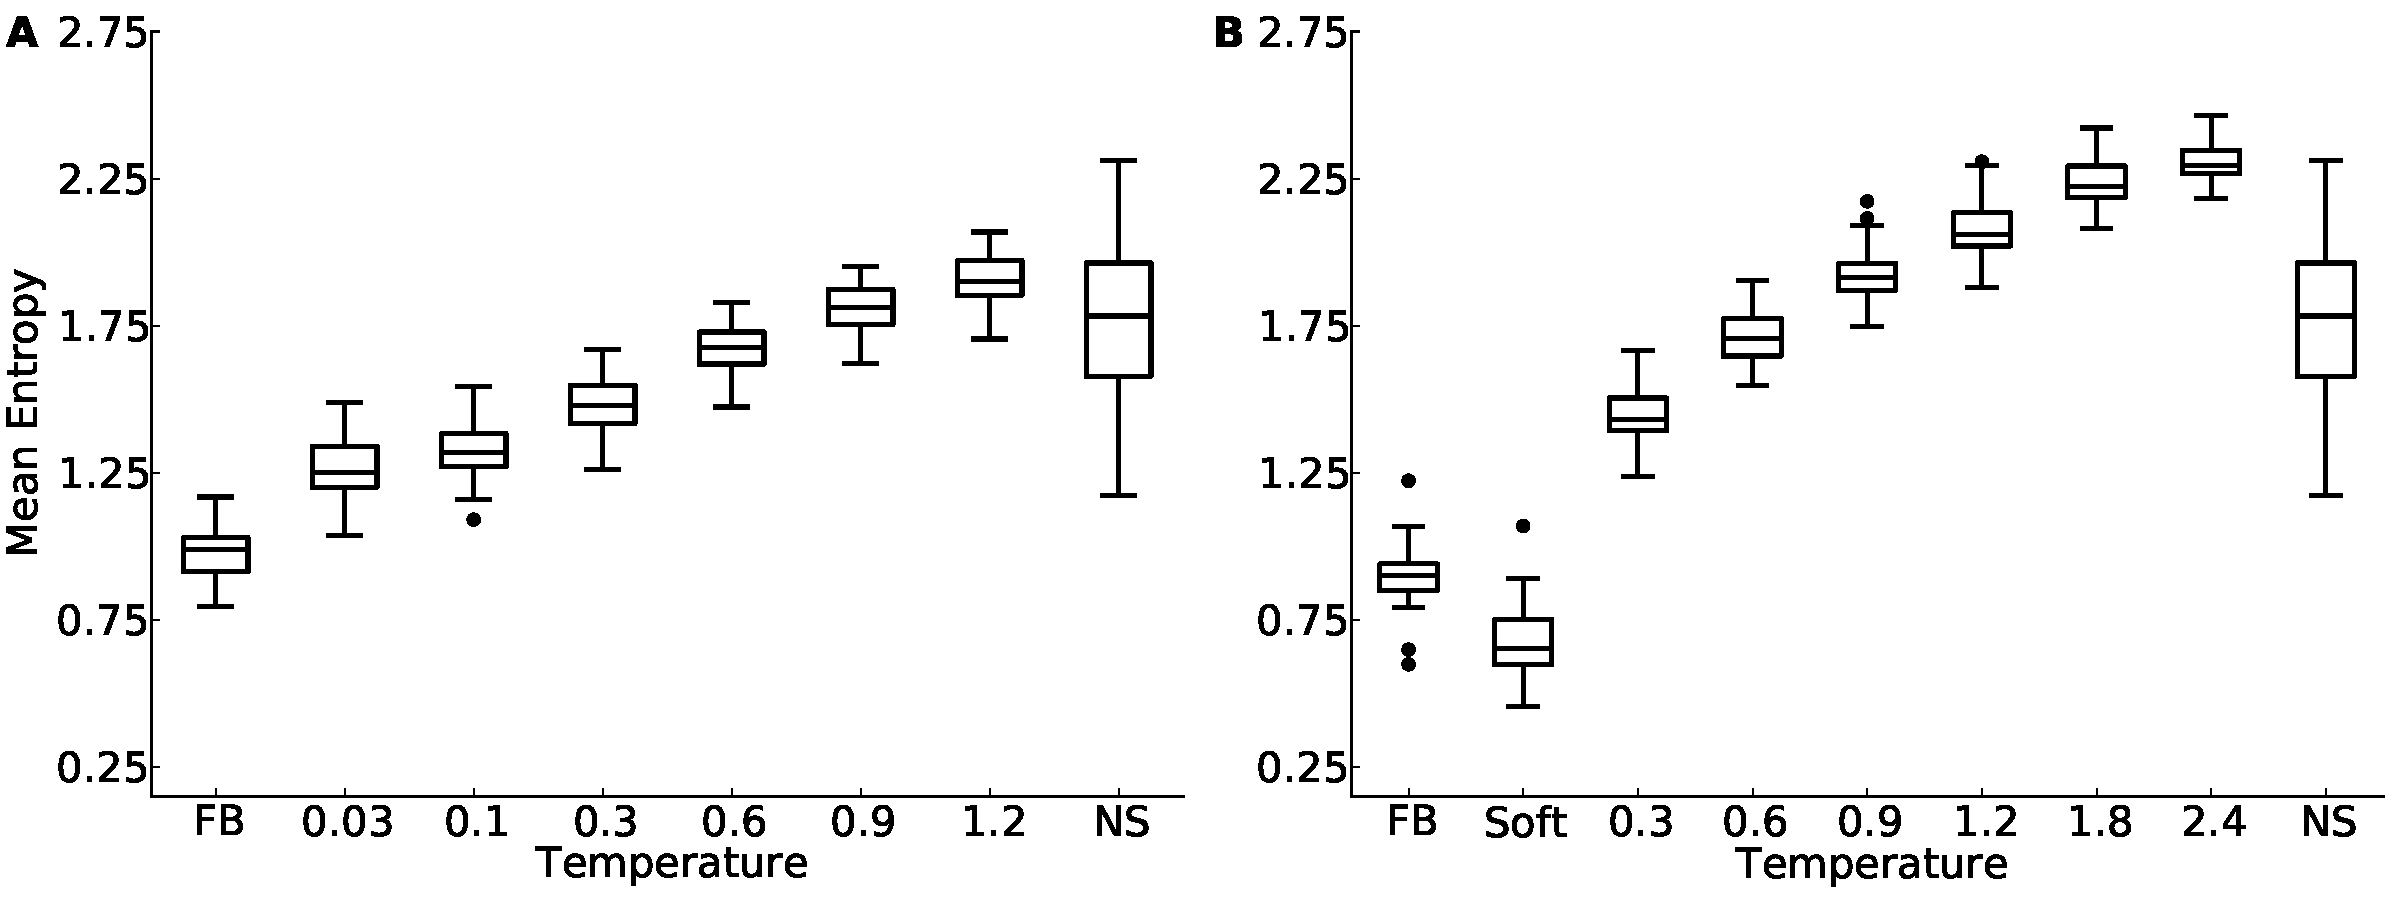
\includegraphics[width = 6in]{figures/Mean_Entropy_vs_Temp_Combo_Boxplot.pdf}} %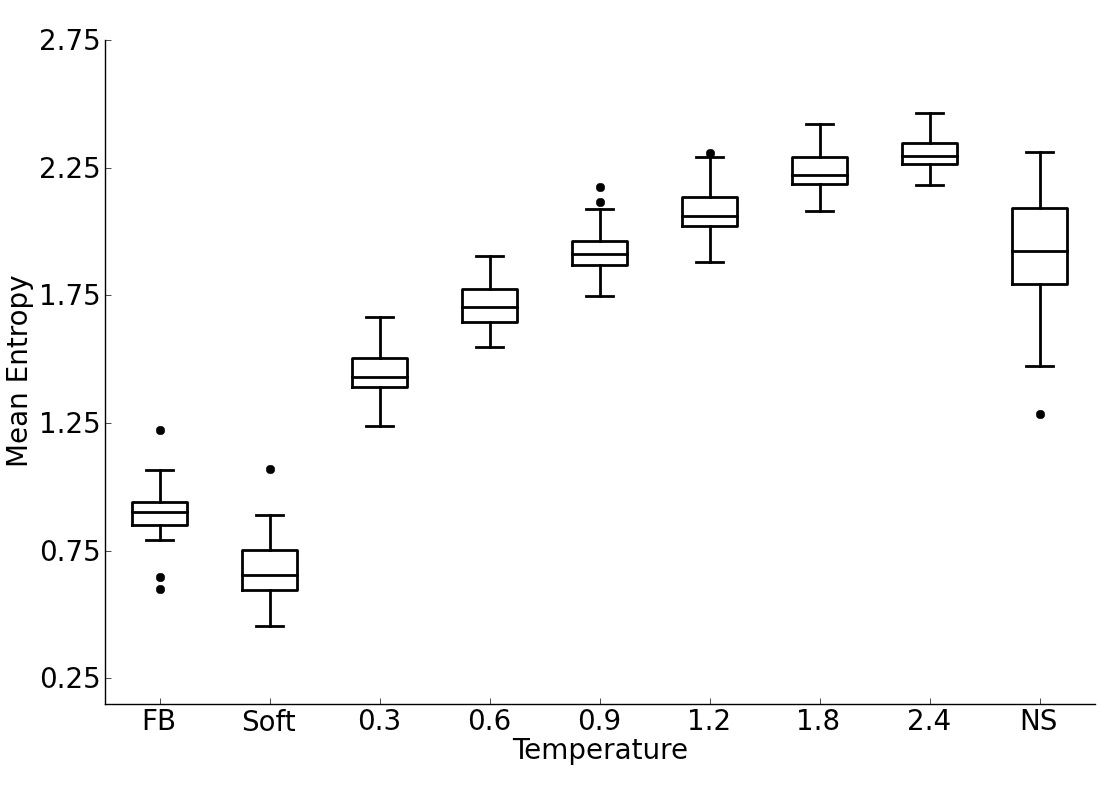
\includegraphics[width = 3in]{figures/Mean_Entropy_vs_Temp_Boxplot_Noah.pdf}}
\caption{Mean site entropy for designed and natural proteins. Each boxplot represents the distribution of mean site entropies within the respective dataset (left: yeast proteins; right: protein domains). ``FB'' refers to fixed-backbone design. Temperature values refer to the design temperature used during the Backrub design method. ``NS'' refers to natural sequences. ``Soft'' refers to the Soft design method. We find generally that more flexible backbones during design allow for more site variability. Intermediate temperatures produce site variabilities most similar to those seen in natural sequences.} Overall, natural sequences in the protein-domains data set are more variable than are those in the yeast-proteins data set.
\label{MeanEntropyComparison}
\end{figure}


\begin{figure}[H]
\centerline{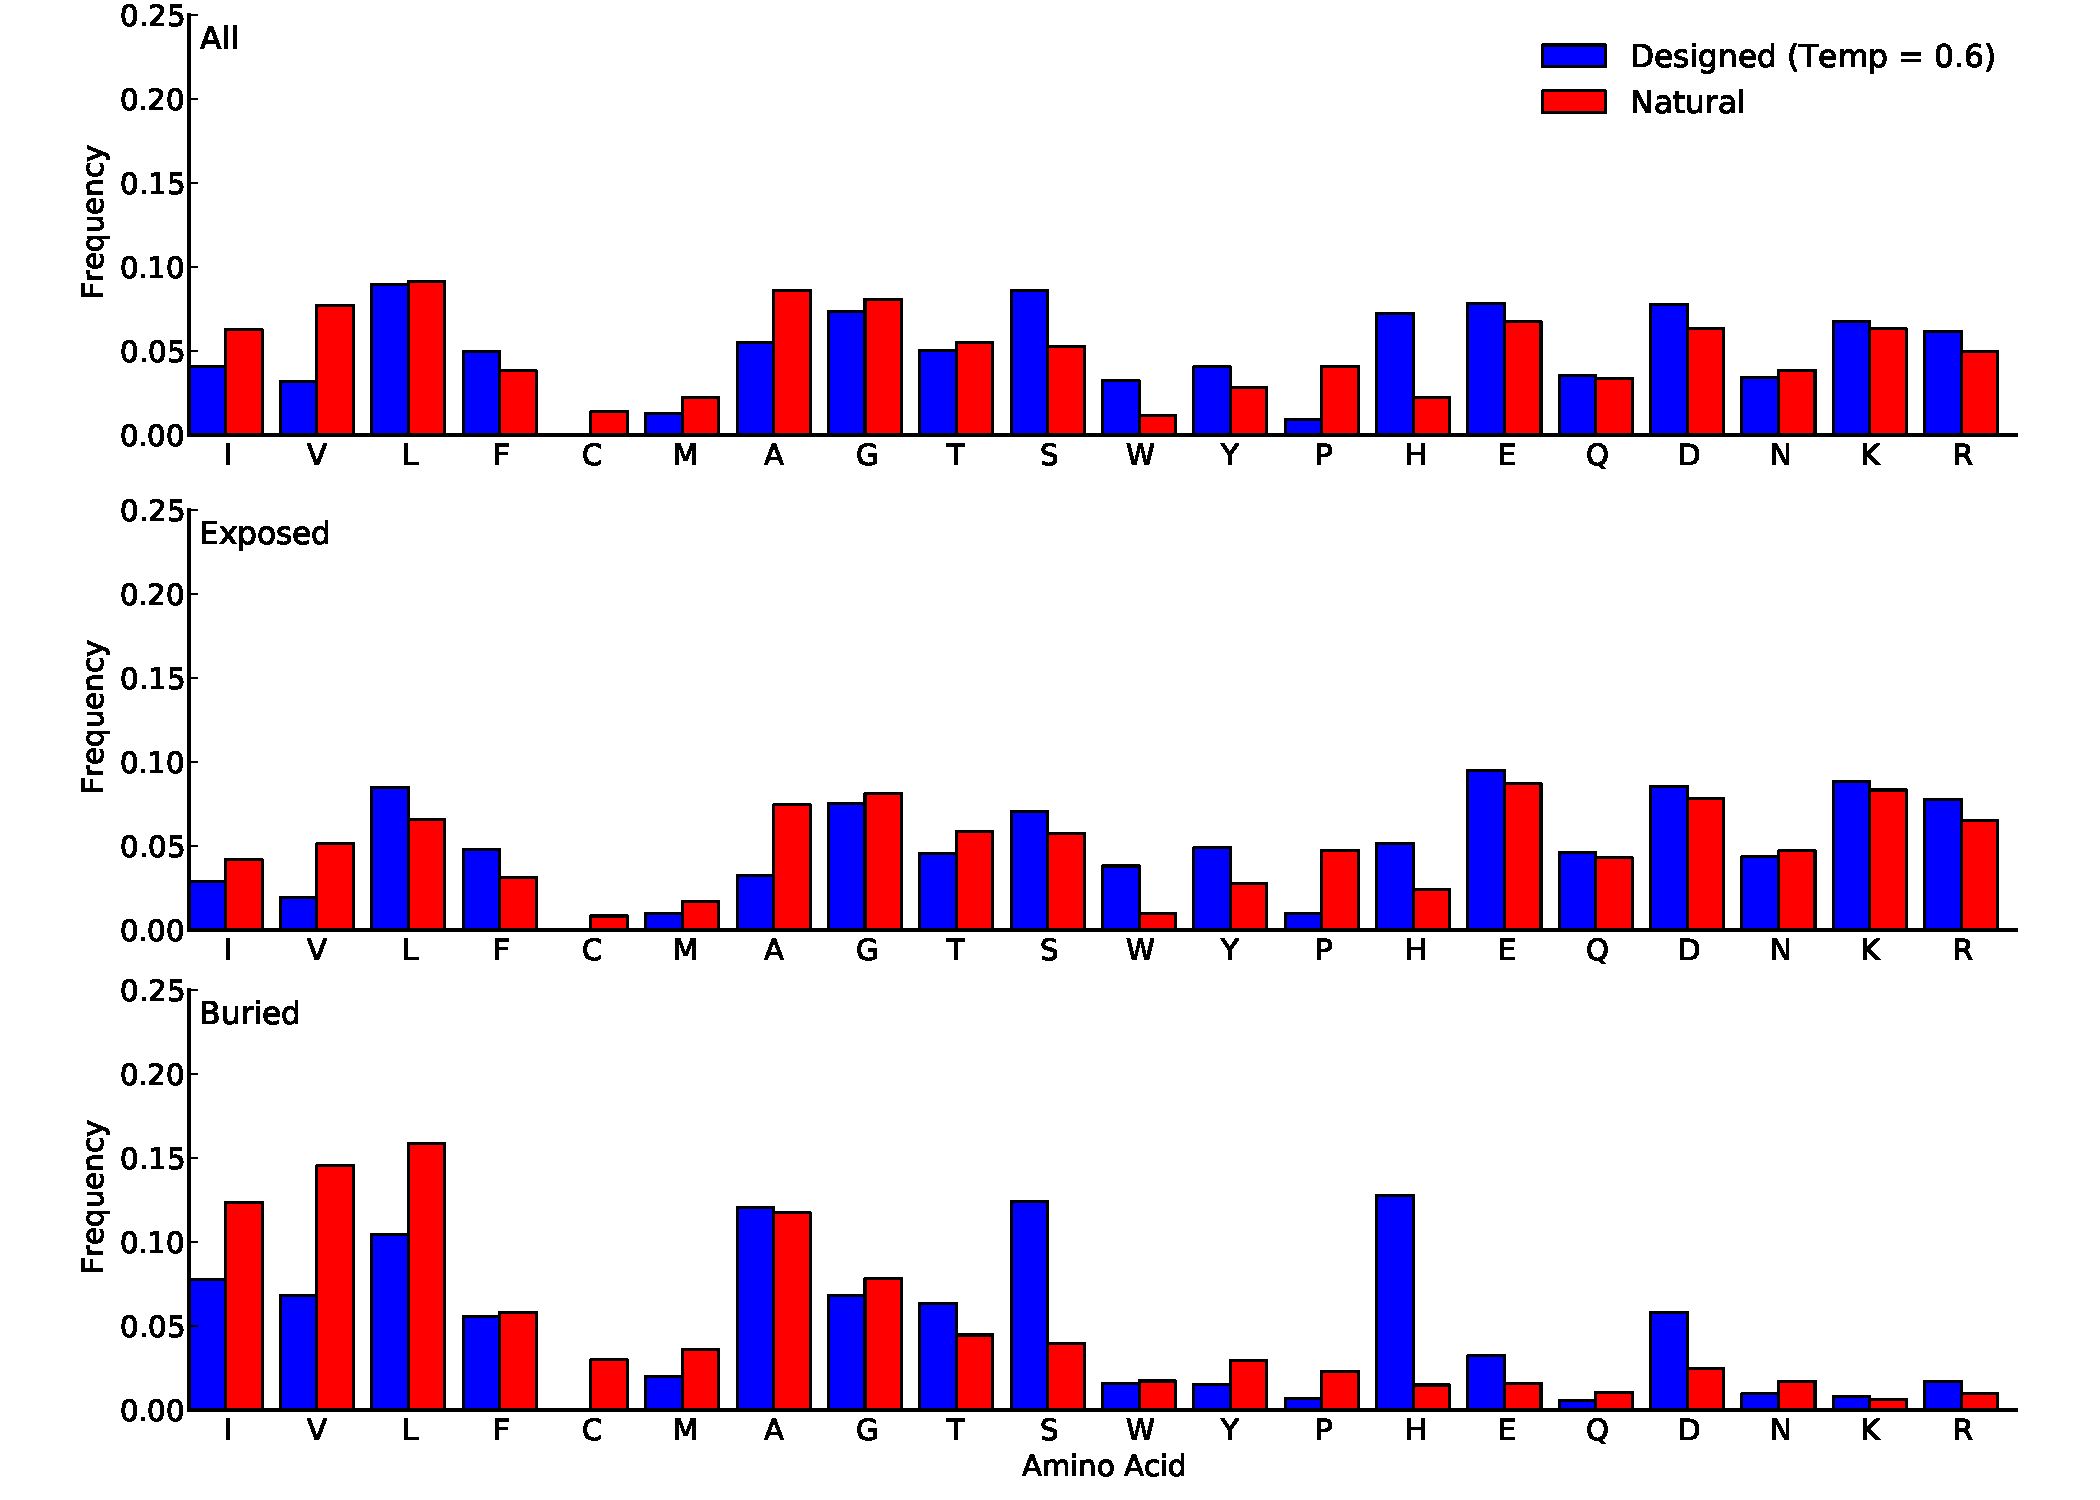
\includegraphics[width = 5in]{figures/Duncan_Freq_Combo_Plots_06.pdf}}
\caption{Amino-acid frequencies in designed and natural proteins. Frequencies were calculated over all sites in all proteins belonging to the yeast-proteins data set. For designed proteins, only flexible-backbone designs with design temperature 0.6 were considered. Top: overall frequencies. Middle: frequencies at exposed sites (defined as sites with $\text{RSA}>0.05$). Bottom: frequencies at buried sites (defined as sites with $\text{RSA}\leq0.05$). {\color{green}\emph{Should we use a different $T$, e.g.\ $T=0.3$?} }  }
\label{AAFreqsYeastProteins}
\end{figure}


\begin{figure}[H]
\centerline{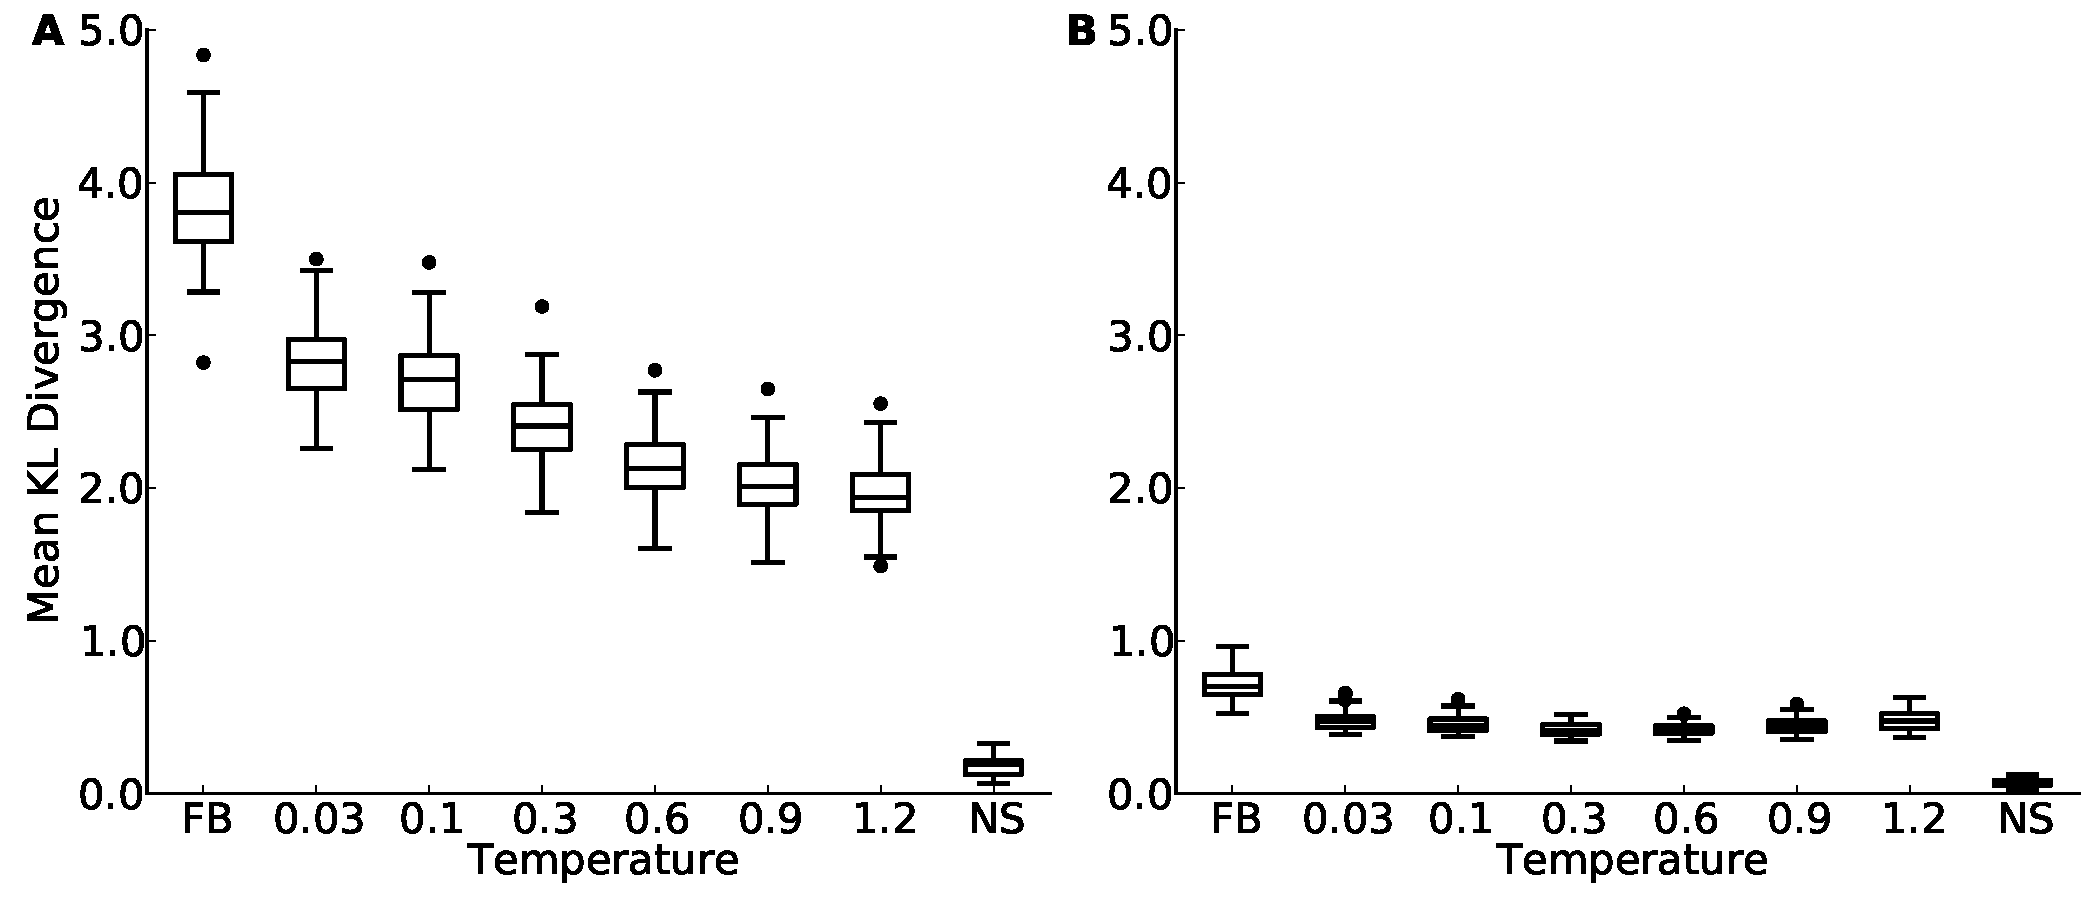
\includegraphics[width = 6in]{figures/Mean_KL_vs_Temp_Boxplot.pdf}}
\caption{Mean Kullback-Leibler (KL) divergence for designed and natural proteins, shown for the yeast-proteins data set. A higher KL divergence indicates that the amino-acid distributions at sites in designed proteins are less similar to the corresponding distributions in the natural proteins. ``FB'' refers to fixed backbone design, and ``NS'' refers to the control case where natural sequences are compared to themselves. (A) KL divergence calculated from the relative frequencies of the 20 amino acids. (B) KL divergence calculated from rank-ordered frequency distributions. The most common amino acid in the reference distribution is compared to the most common amino acid in the focal distribution, the same is done for the second-most common amino acid, and so on, irrespective of the type of amino acids.}
\label{AADisFig1}
\end{figure}


\begin{figure}[H]
\centerline{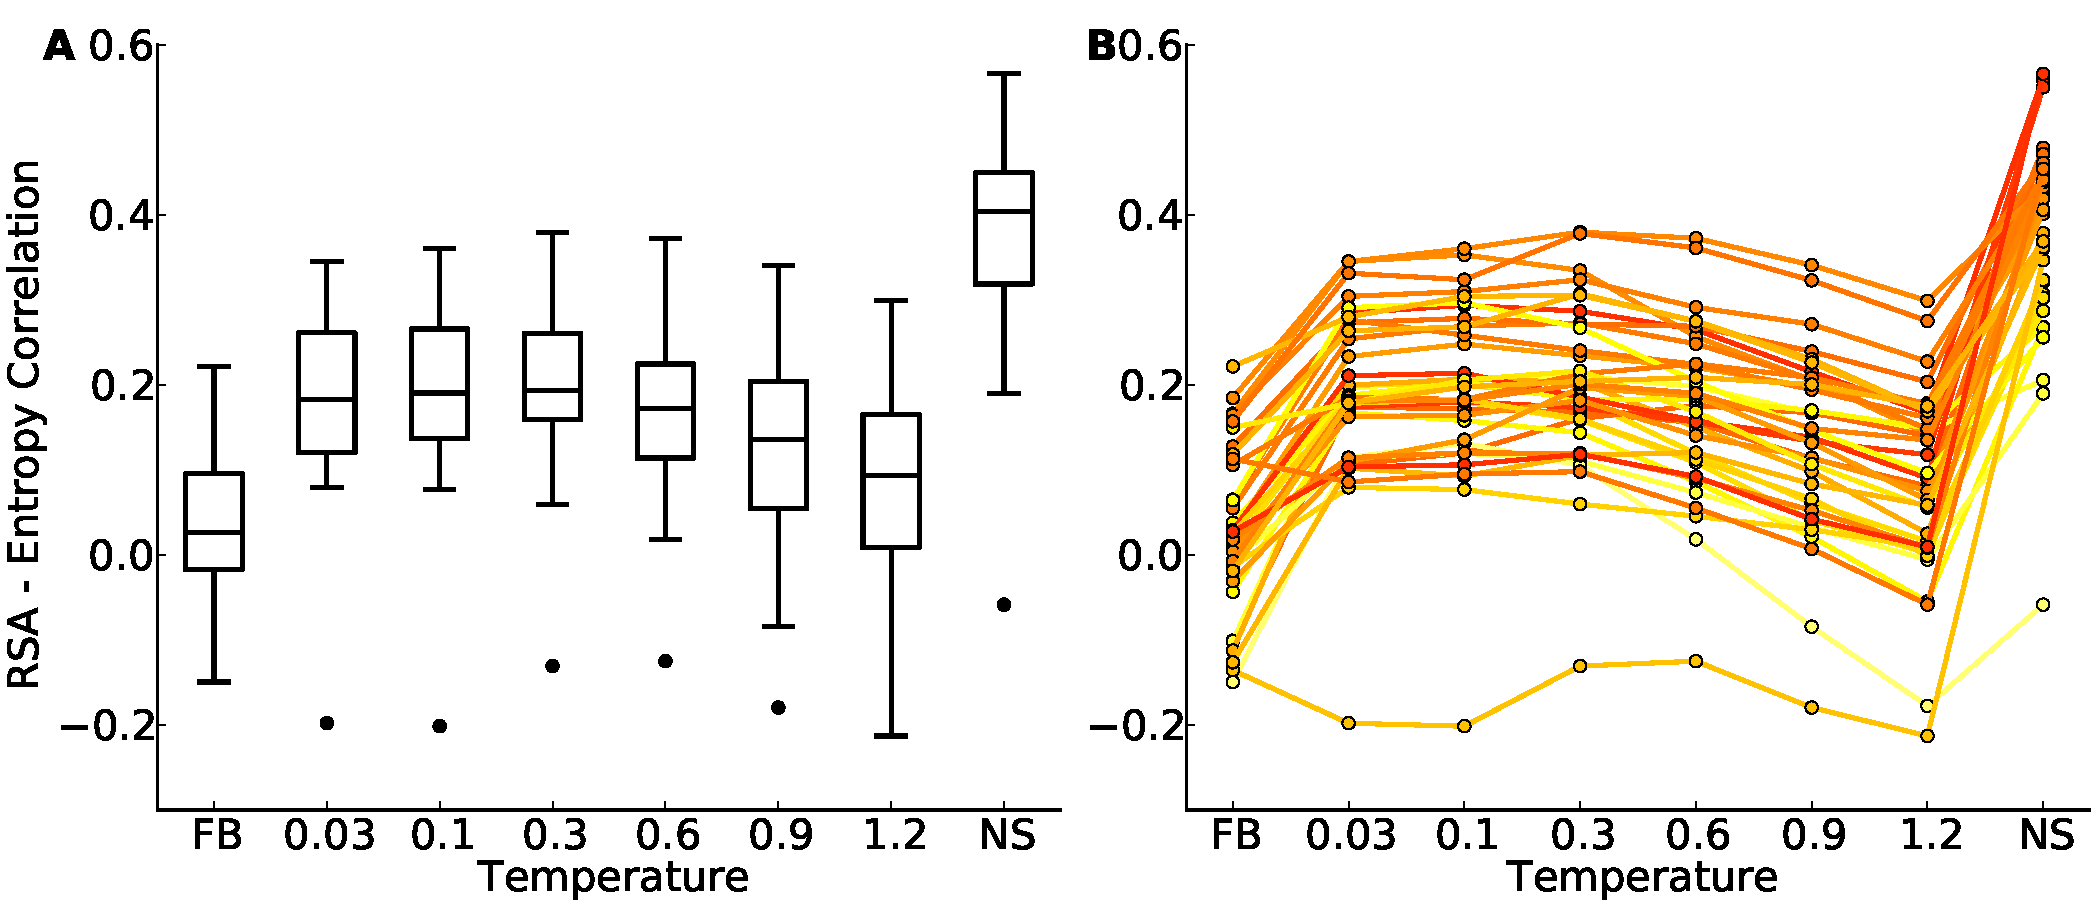
\includegraphics[width = 6in]{figures/Cor_Mean_Entropy_RSA_Combination_Plot.pdf}}
\caption{Distributions of correlation coefficients between site entropy and RSA, for the yeast-proteins data set. ``FB'' indicates fixed-backbone design, and ``NS'' indicates natural sequences. (A) Distributions represented as boxplots. (B) Correlation coefficients for individual proteins. Lines connect identical structures in the different design conditions. The color shading represents the strength of the correlation for the natural sequence alignment. In general, natural proteins display a stronger correlation between site entropy and RSA than designed proteins.}
\label{Correlation_figure}
\end{figure}


\begin{figure}[H]
\centerline{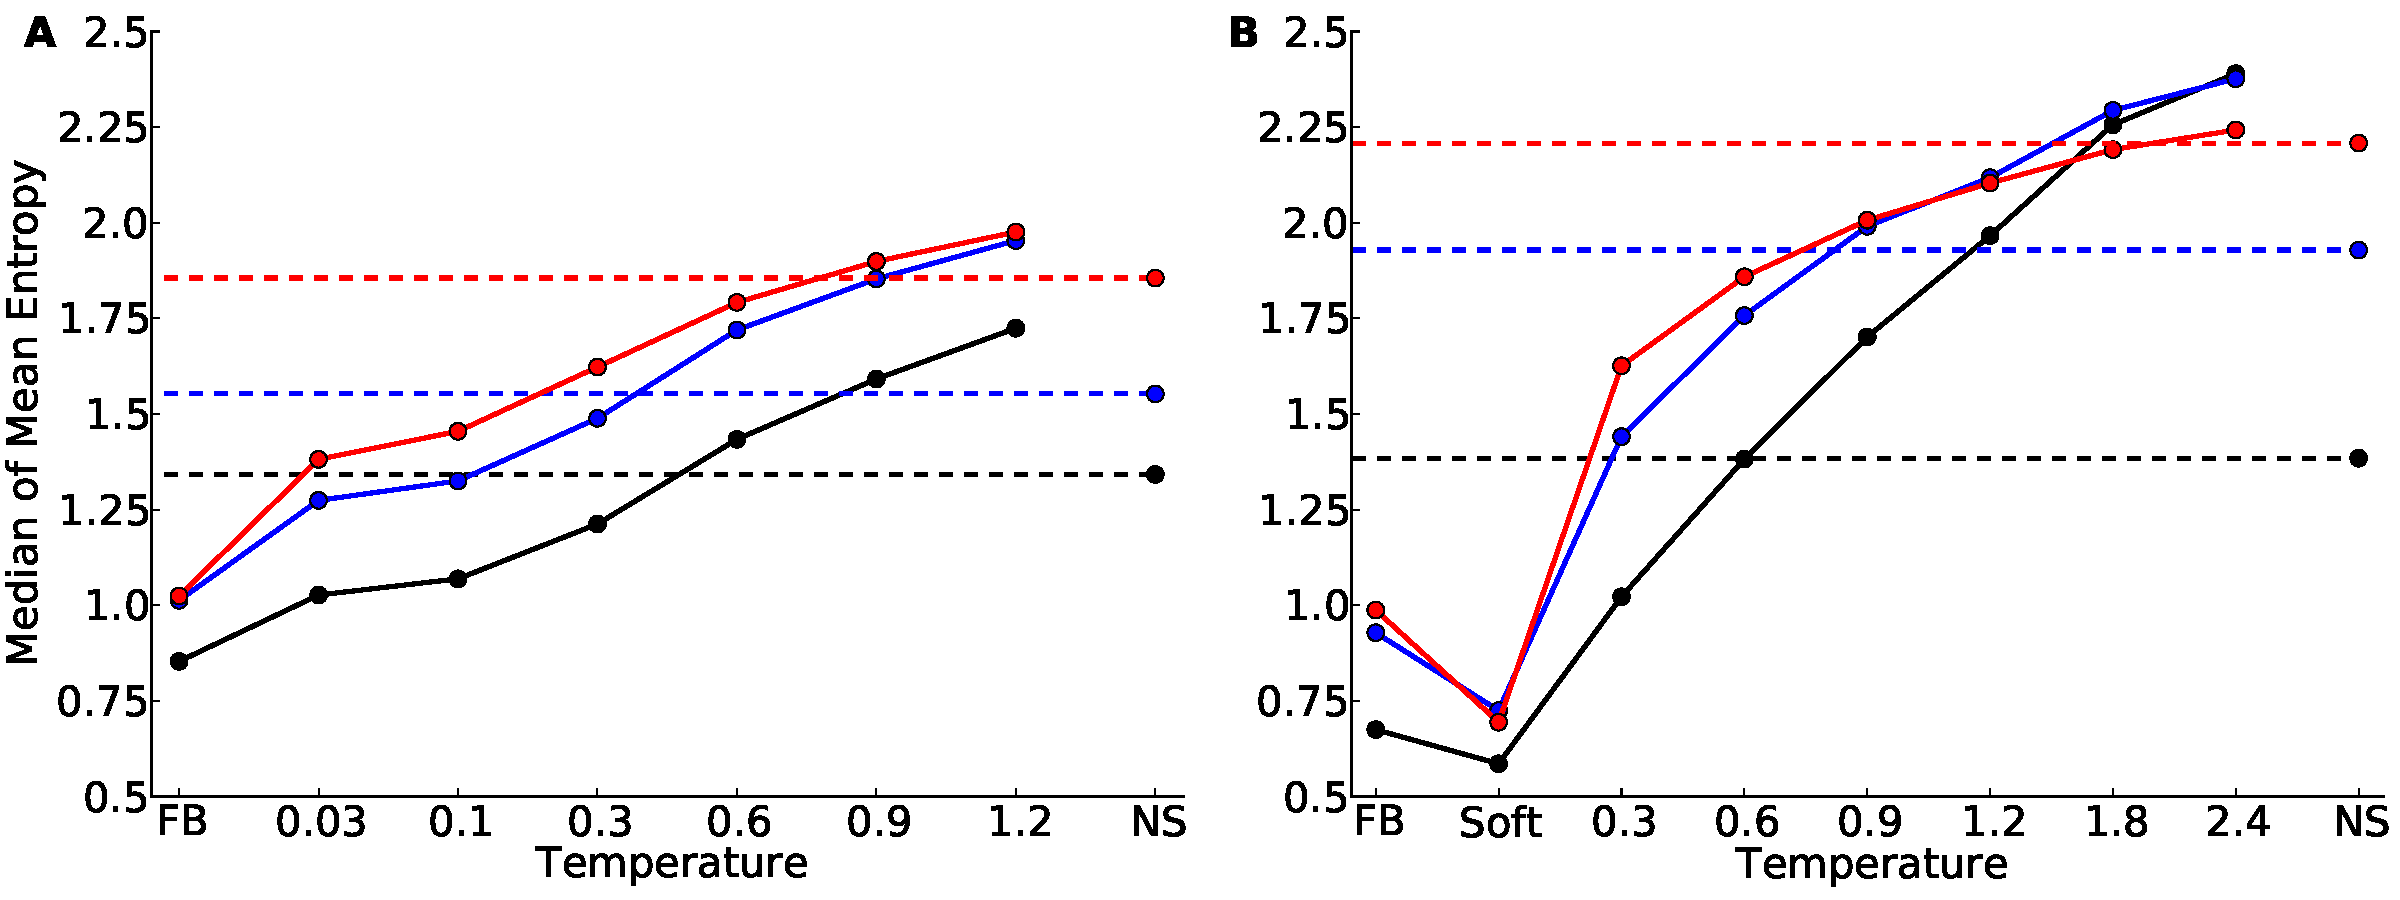
\includegraphics[width = 6in]{figures/Mean_Entropy_Position_Lineplot_Combo.pdf}}
\caption{Median of the distribution of mean sequence entropies for designed and natural sequences, calculated separately for buried (black), partially buried (blue), and exposed (red) residues (left: yeast proteins; right: protein domains). We defined buried sites as those with $\text{RSA}\leq 0.05$, partially buried as those with $0.05<\text{RSA}\leq0.25$, and exposed as those with $\text{RSA}>0.25$. Dashed lines indicate the corresponding median for natural sequence alignments. Note that for buried (black) and partially buried (blue) residues, the temperatures at which natural site variability and design variability match are comparable. By contrast, for exposed residues, a higher design temperature is required for the design variability to match the natural site variability.}
\label{Mean_Entropy_Surface_Core}
\end{figure}


\begin{figure}[H]
\centerline{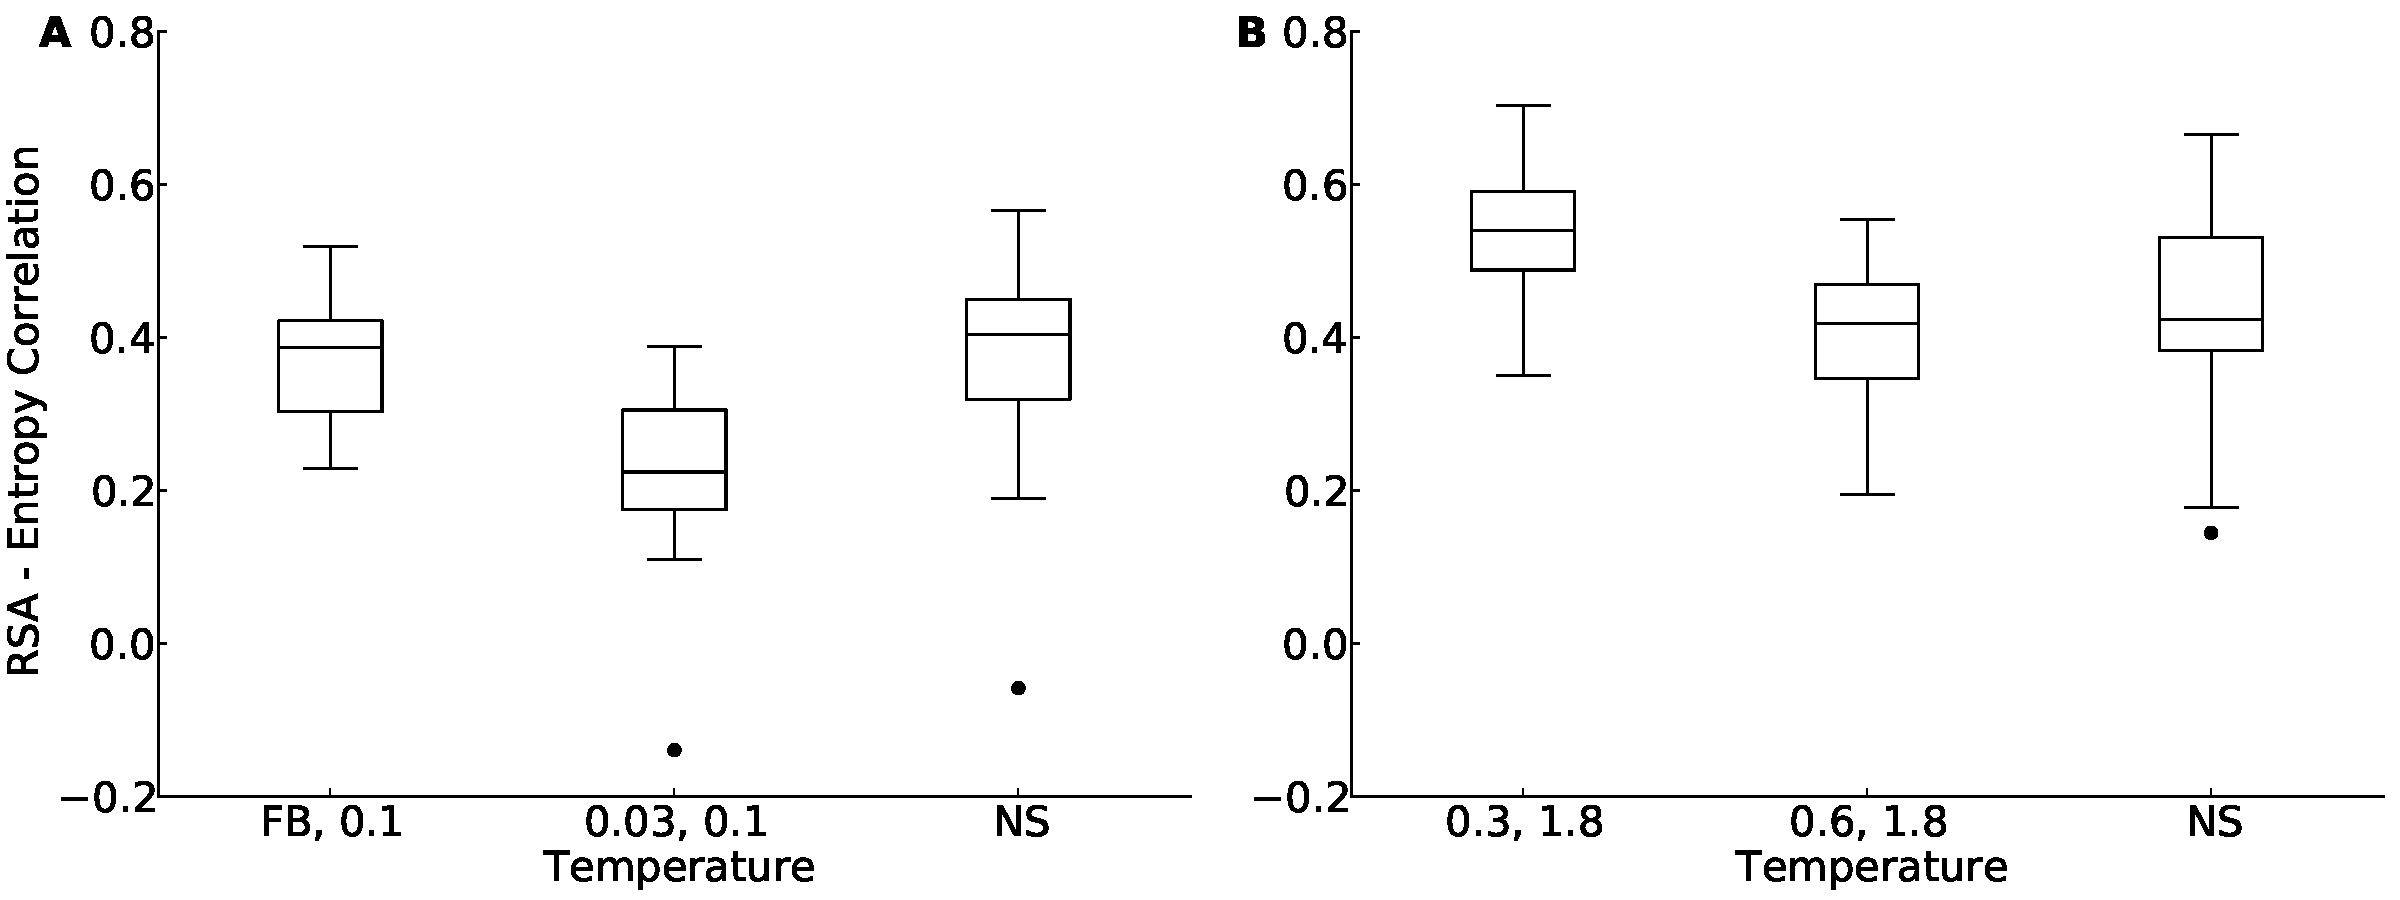
\includegraphics[width = 6in]{figures/Combo_Mixed_Temp_Correlation_Plot.pdf}}
\caption{Distribution of correlation coefficients between RSA and site entropy for hybrid designs and for natural proteins. {\color{red}For the hybrid designs, buried and partially buried sites were taken from sequences designed at one temperature, and exposed sites were taken from sequences designed at a different temperature. For the hybrid designs, the correlation coefficients were similar to those of natural sequences (paired $t$ test,  $P=0.532$ (T = FB, 0.1)  and  $P= 8.09 $ $\times$ $10^{-8}$ (T = 0.03, 0.1) [yeast proteins], $P= 5.74$  $\times$ $10^{-5}$ (T = 0.3, 1.8) and $P= 0.123$ (T = 0.6, 1.8)  [protein domains])}}
\label{Mixed_RSA_Entropy}
\end{figure}


\cleardoublepage

\section{Supporting Figures}

\centerline{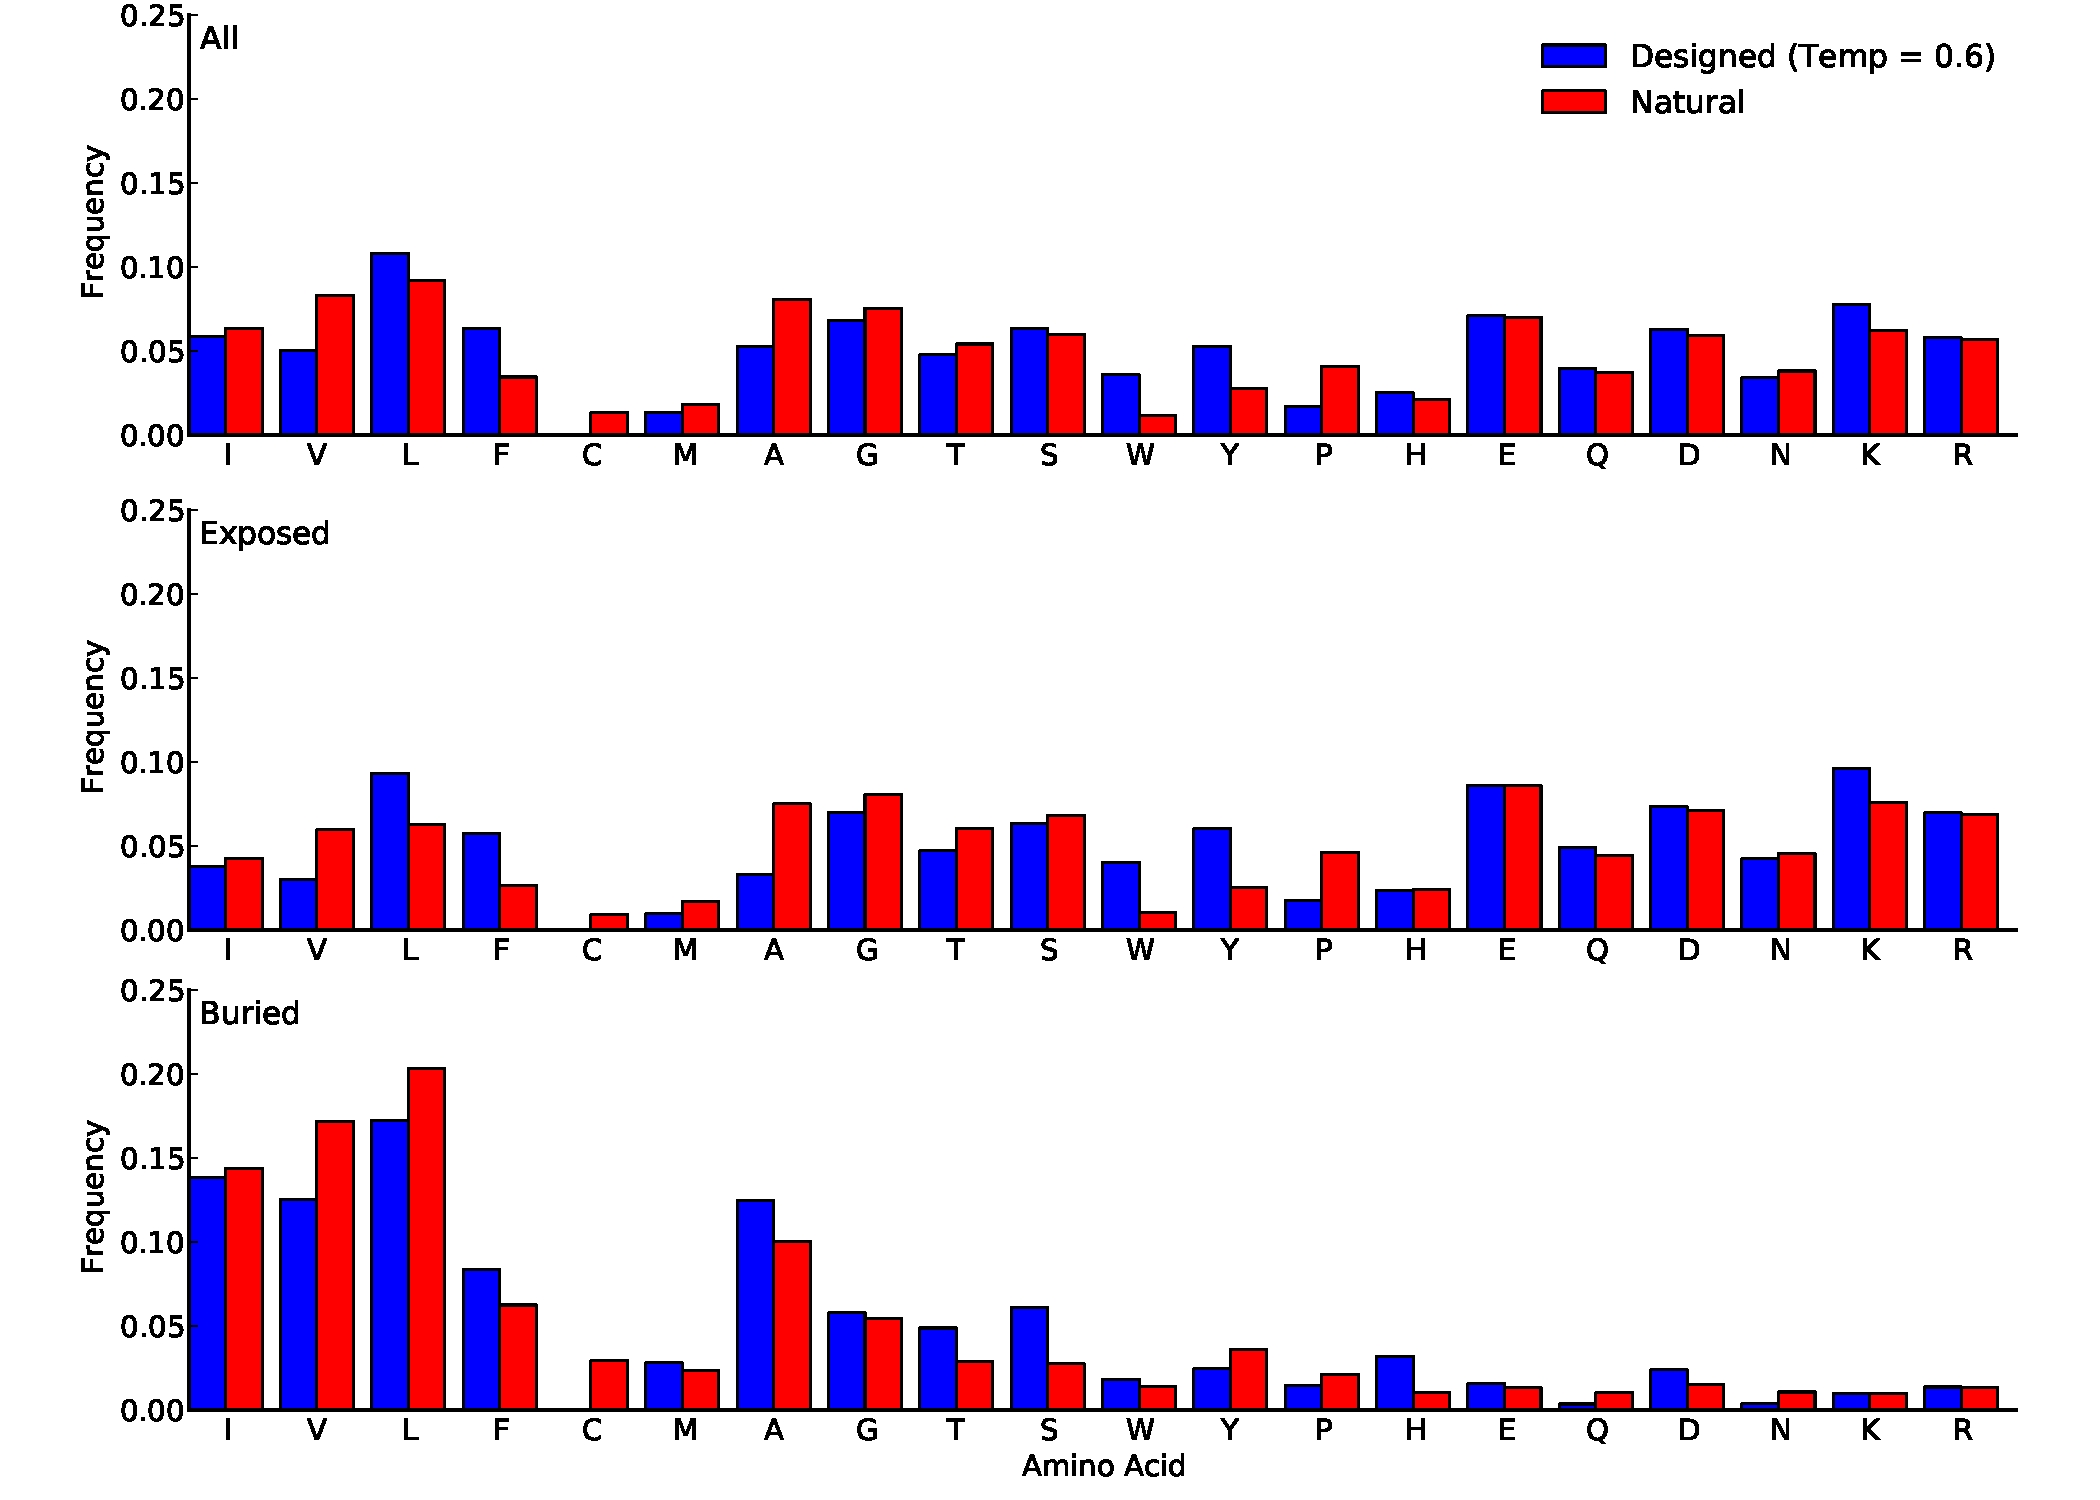
\includegraphics[width = 5in]{figures/Noah_Freq_Combo_Plots_06.pdf}}

\noindent Figure S1. Amino-acid frequencies in designed and natural proteins. Frequencies were calculated over all sites in all proteins belonging to the protein-domains data set. For designed proteins, only flexible-backbone designs with design temperature 0.6 were considered. Top: overall frequencies. Middle: frequencies at exposed sites (defined as sites with $\text{RSA}>0.05$). Bottom: frequencies at buried sites (defined as sites with $\text{RSA}\leq0.05$) {\color{blue}\emph{Once again should this be a different temperature?} } .

\customlabel{AAFreqsProteinDomains}{S1}

\newpage

\centerline{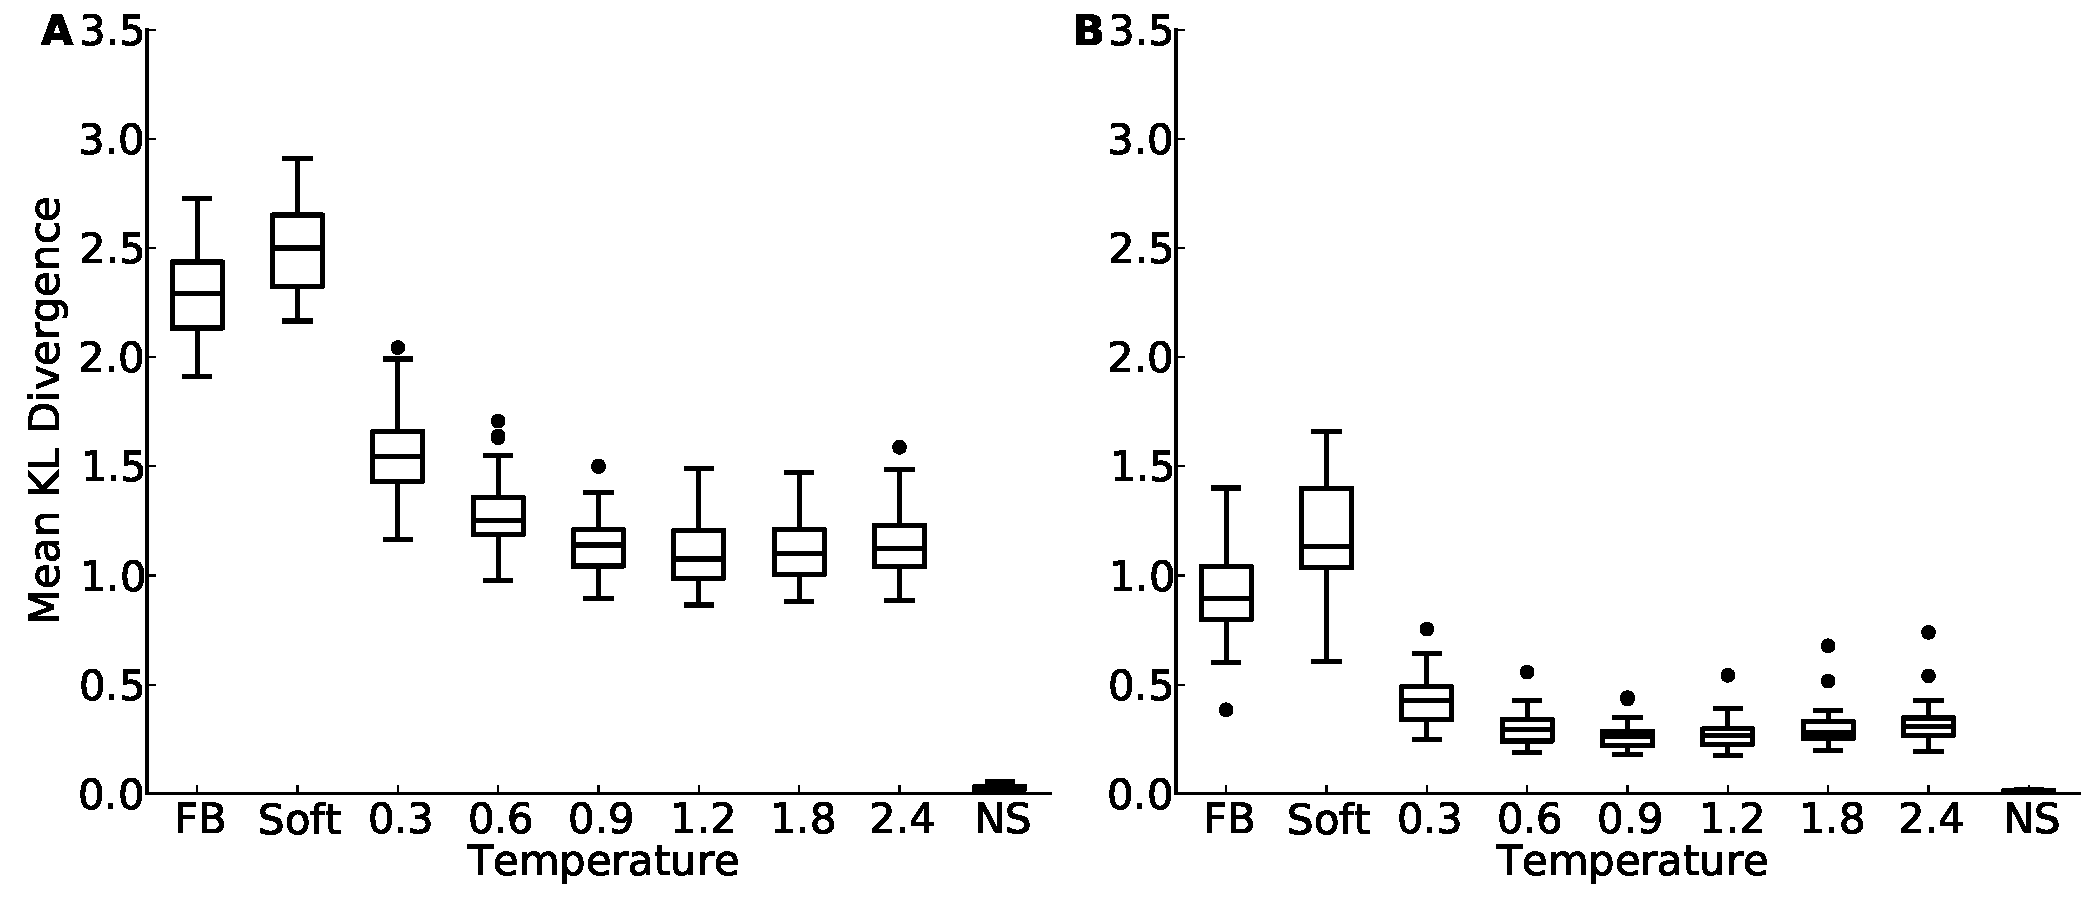
\includegraphics[width = 6in]{figures/Mean_KL_vs_Temp_Boxplot_Noah.pdf}}
\noindent Figure S2. Mean Kullback-Leibler (KL) divergence for designed and natural proteins, shown for the yeast-proteins data set. A higher KL divergence indicates that the amino-acid distributions at sites in designed proteins are less similar to the corresponding distributions in the natural proteins. ``FB'' refers to fixed backbone design, and ``NS'' refers to the control case where natural sequences are compared to themselves. (A) KL divergence calculated from the relative frequencies of the 20 amino acids. (B) KL divergence calculated from rank-ordered frequency distributions. The most common amino acid in the reference distribution is compared to the most common amino acid in the focal distribution, the same is done for the second-most common amino acid, and so on, irrespective of the type of amino acids.

\customlabel{NoahAADisFig1}{S2}

\newpage


\centerline{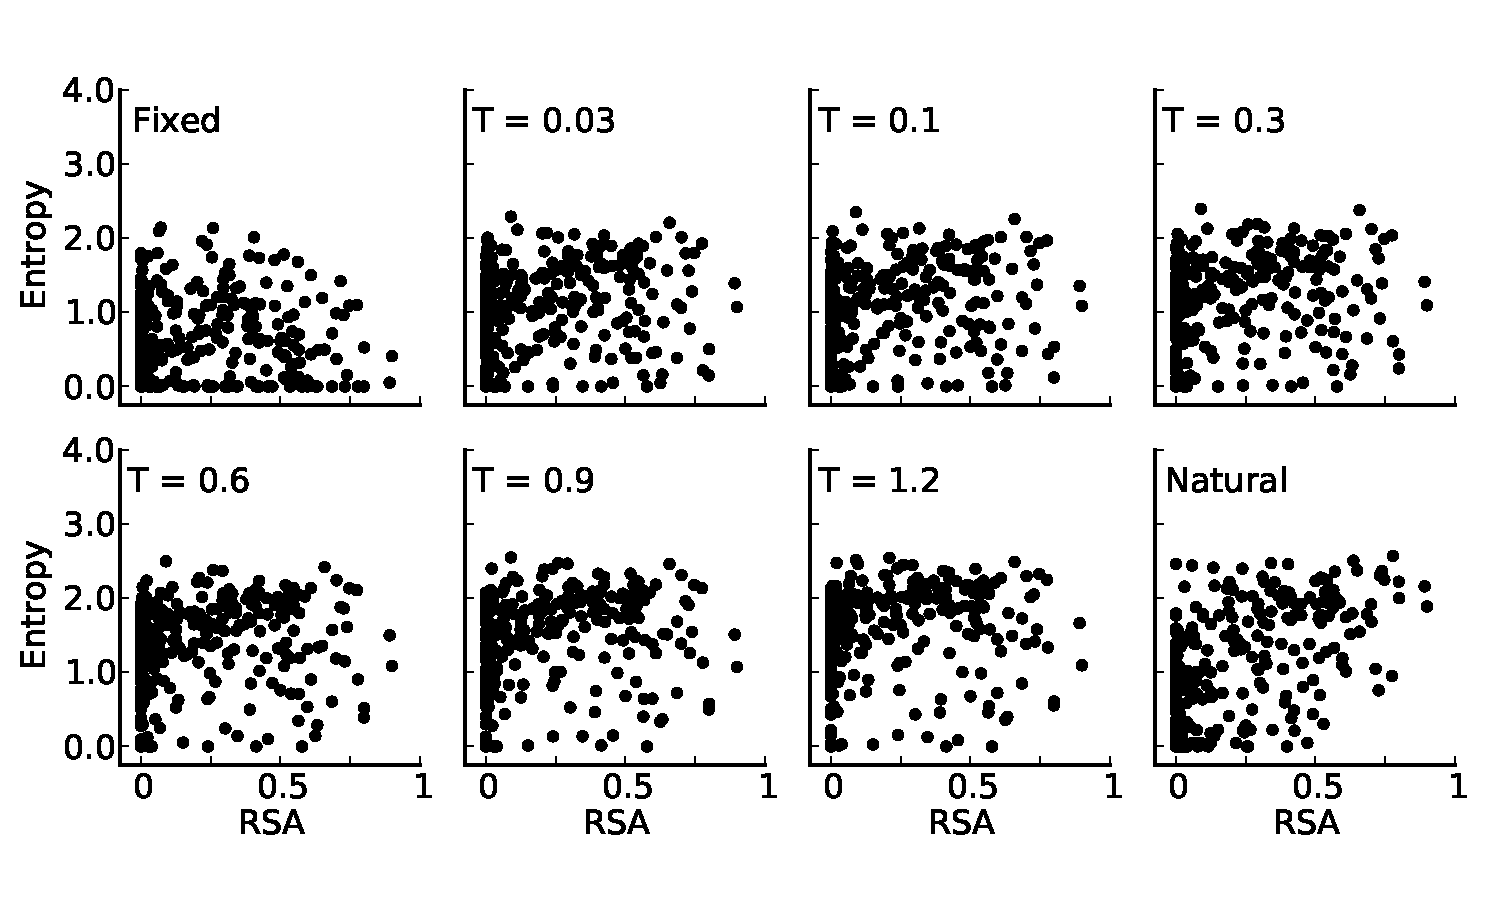
\includegraphics[width = 6.5in]{figures/RSA_vs_Entropy_1PV1_Combination_Plot.pdf}}

\noindent Figure S3. Site entropy versus Relative Solvent Accessibility (RSA) for designed and natural sequence alignments of the protein S-formylglutathione hydrolase (PDB: 1PV1, chain A). {\color{blue}\emph{[Methods?$\rightarrow$ ]} RSA values are calculated from the published PDB structure.} Natural sequences exhibit a clear trend of higher site variability at higher RSA values. The flexible backbone designs exhibit a similar trend but the fixed backbone designs do not.
\customlabel{Entropy_vs_RSA_example}{S3}

\newpage

\centerline{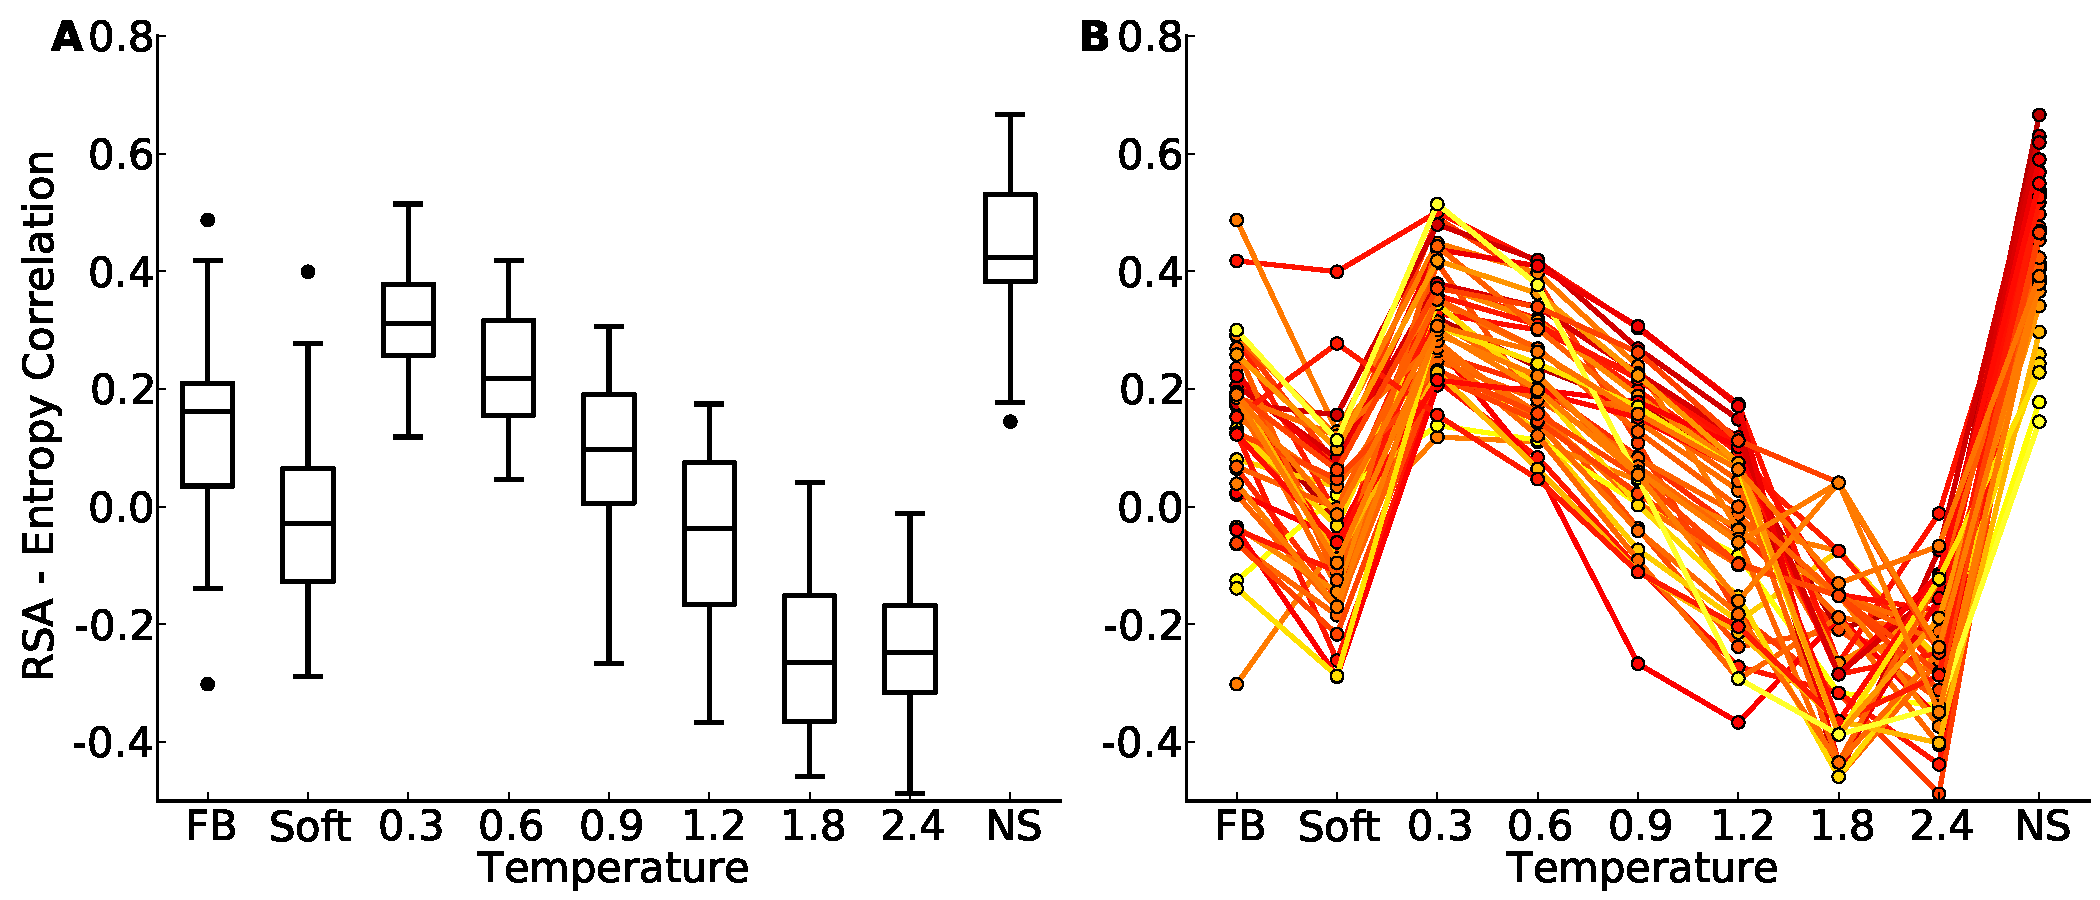
\includegraphics[width = 6in]{figures/Cor_Mean_Entropy_RSA_Combination_Plot_Noah.pdf}}
\noindent Figure S4. Distributions of correlation coefficients between site entropy and RSA, for the yeast-proteins data set. ``FB'' indicates fixed-backbone design, ``Soft'' indicates soft backbone design, and ``NS'' indicates natural sequences. (A) Distributions represented as boxplots. (B) Correlation coefficients for individual proteins. Lines connect identical structures in the different design conditions. The color shading represents the strength of the correlation for the natural sequence alignment. In general, natural proteins display a stronger correlation between site entropy and RSA than designed proteins.

\customlabel{Correlation_figure_Noah}{S4}

\newpage

% \centerline{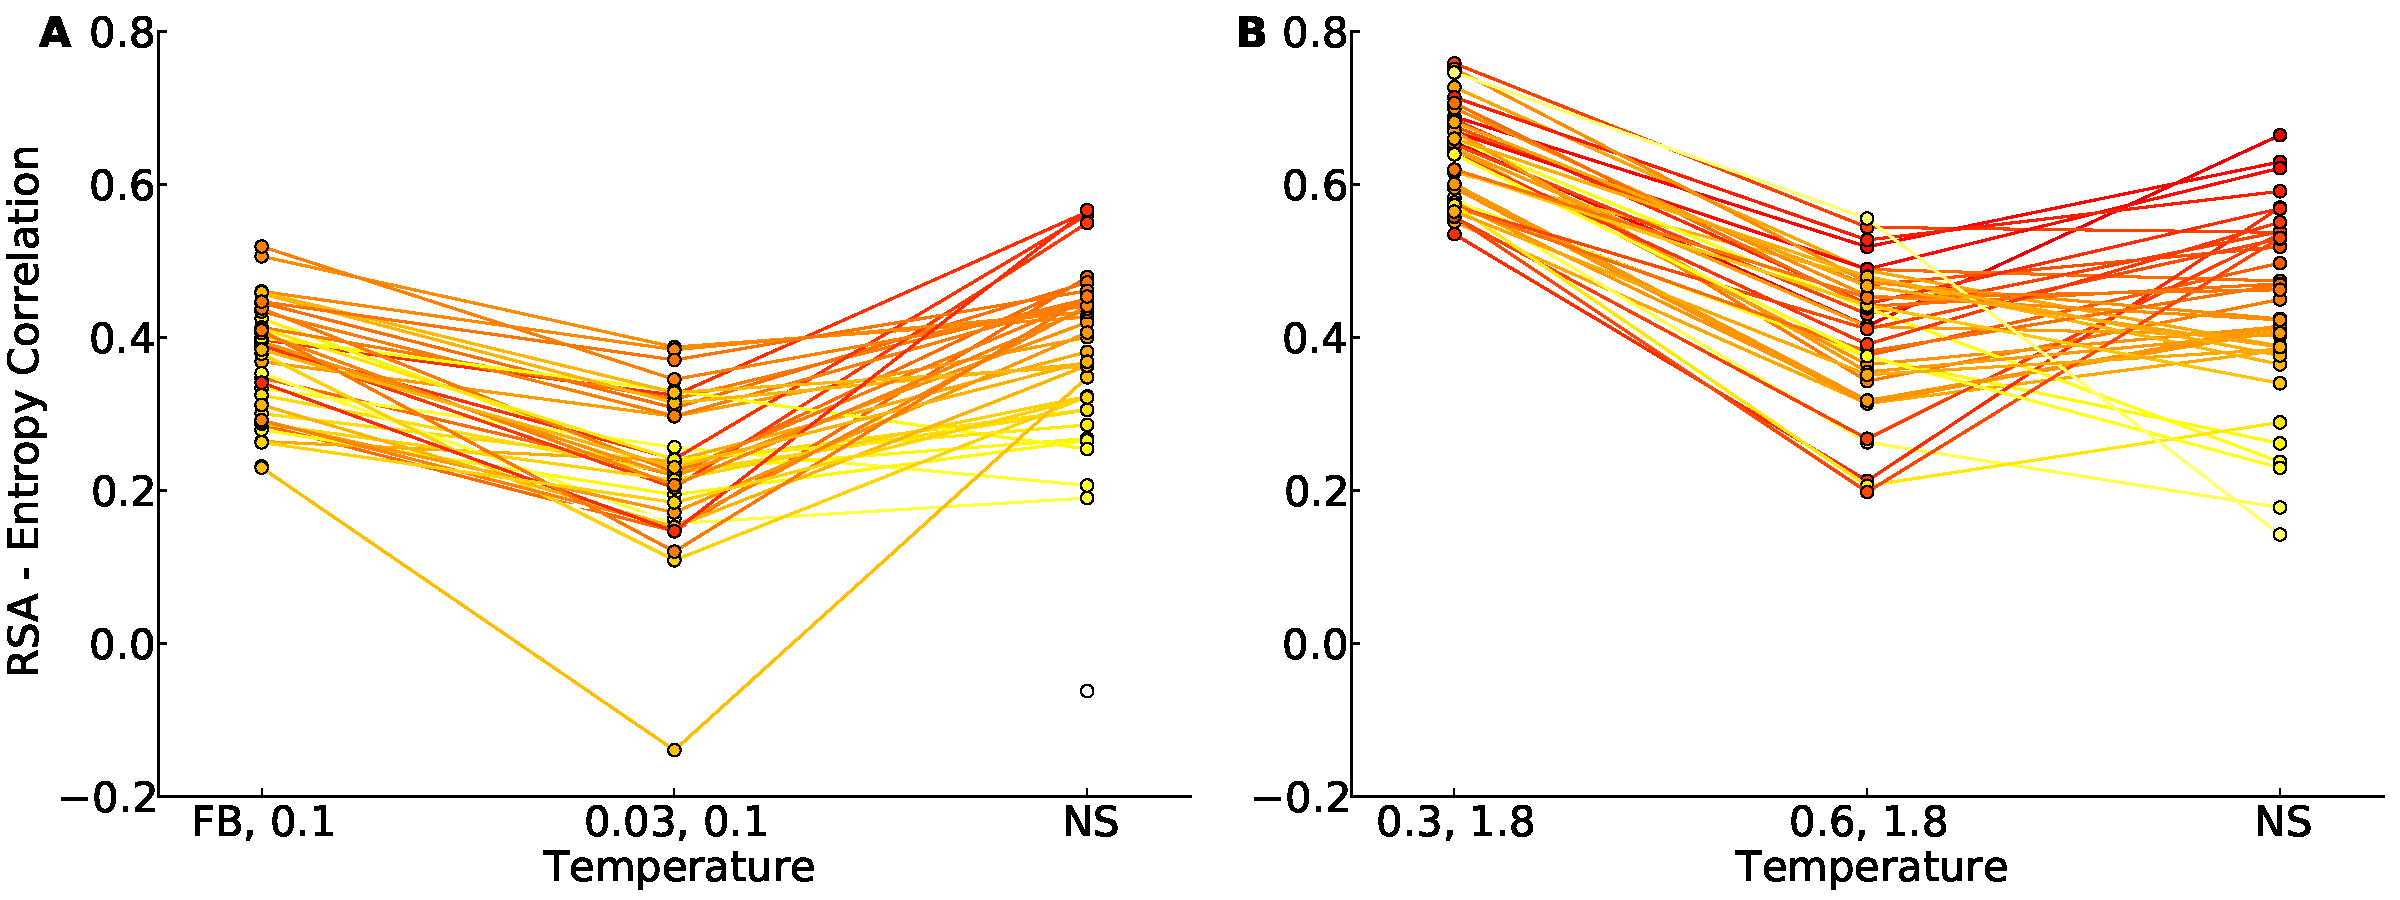
\includegraphics[width = 6in]{figures/Combo_Lineplot_Mixed_Temp_Correlation_Plot.pdf}}
% \noindent Figure S4.  Distribution of  the correlation coefficients between RSA and site entropy for hybrid designed and natural proteins. Colors correspond to the magnitude of the correlation coefficient in the natural proteins. Hybrids were created by taking sequences for buried residues and partially residues from one temperature and exposed residues from another temperature (left: yeast proteins, right: protein domains). "NS" refers to the natural sequences and "FB" refers to fixed backbone. 
% \customlabel{Combo_Mixed_Entropy_Lineplot}{S5}
% 
% \newpage


\centerline{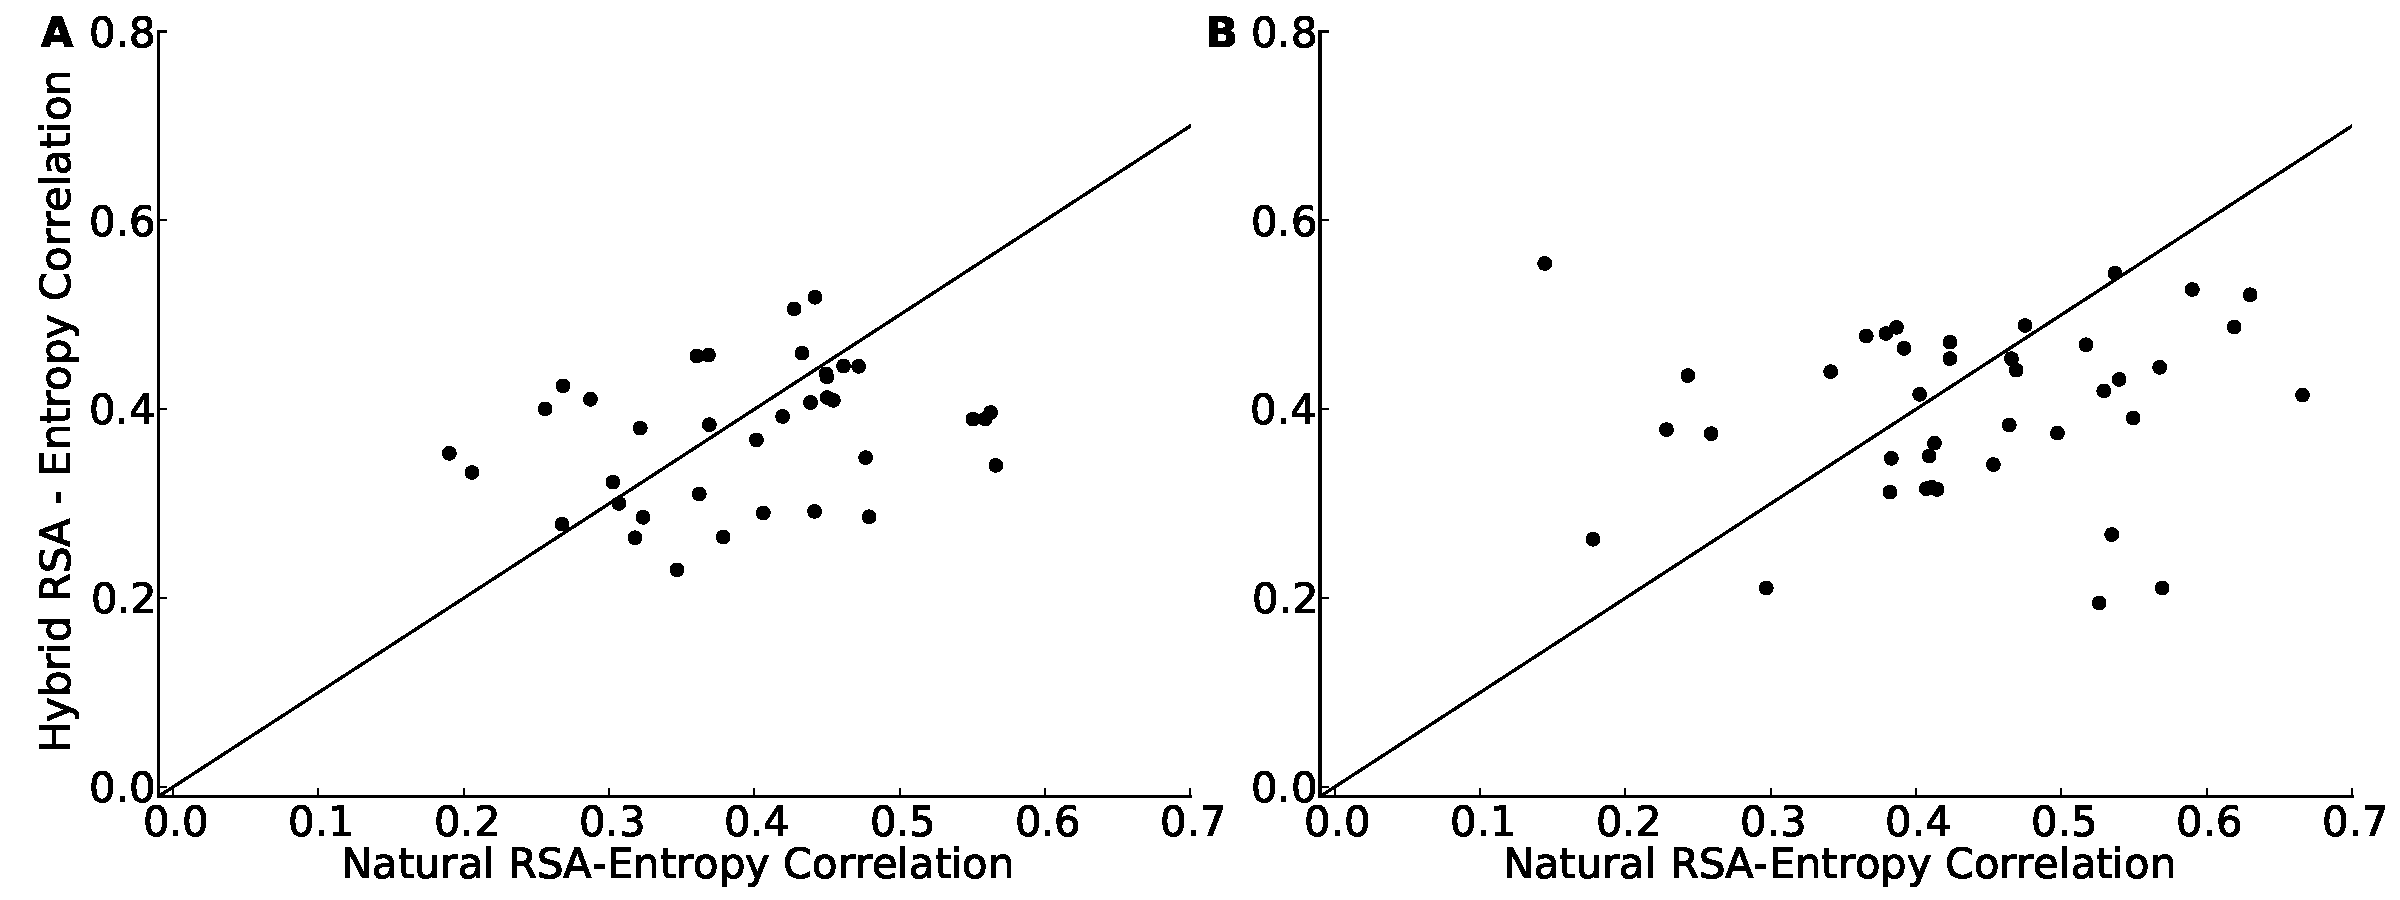
\includegraphics[width = 6in]{figures/Combo_Lineplot_Mixed_Temp_Correlation_Lineplot.pdf}}
\noindent Figure S5. Correlation coefficients between RSA and site entropy for hybrid designs and natural proteins. For the hybrid designs, buried and partially buried sites were taken from proteins designed with a fixed backbone (yeast proteins) or a temperature of $T = 0.6$ (protein domains). Exposed residues were taken from proteins designed with a temperature of $ T =  0.1$ (yeast proteins) or $T = 1.8$ (protein domains). The solid line indicates $y=x$. Note that while the range of correlation values in hybrid designs generally matches the range of values in natural alignments, predictions for specific proteins are not that accurate.

\customlabel{Mixed_Entropy_Correlation_Plot}{S5}

\end{document}